\chapter{Differential Forms}

\section{Multilinear Algebra}

\begin{definition}
    Let $V$ be a vector space. Let $V^k=V\times \cdots \times V$ denote the set of all k-tuples $(v_1,\cdots,v_k)$ of vectors of $V$. A function $f:V^k\longrightarrow\R$ is said to be \underline{linear in the i-th variable} if given vectors $v_j$ for $j\neq i$, the function $T:V\longrightarrow \R$ defined by $$T(v)=f(v_1,\cdots,v_{i-1},v,v_{i+1},\cdots,v_k)$$ is linear. The function $f$ is said to be \underline{multilinear} if it is 
    linear in the i-th variable for each i. Such a function $f$ is also called a \underline{k-tensor on $V$}. We denote the set of all k-tensors on $V$ by the symbol $\mathcal{L}^k(V)$. If $k=1$, then $\mathcal{L}^1(V)$ is just the set of all linear transformations $f:V\longrightarrow\R$. It is also called the \underline{dual space} of $V$ and denoted by $V^*$.
\end{definition}

\begin{theorem}
    The set of all k-tensors on $V$ constitutes a vector space if we define 
    \begin{enumerate}
        \item $(f+g)(v_1,\cdots,v_k)=f(v_1,\cdots,v_k)+g(v_1,\cdots,v_k)$
        \item $(cf)(v_1,\cdots,v_k)=c(f(v_1,\cdots,v_k))$
    \end{enumerate}
\end{theorem}

\noindent\textbf{Example}: Tensors we already know.
\begin{itemize}
    \item 1-tensor.
    \begin{enumerate}
        \item Given the vector space $V$, equipped with an inner product. Define $f:V\longrightarrow\R$ by 
        $$f(v)=\innerp{v}{w}\text{ where $w$ is a fixed vector}$$
        \item Given the vector space $V$ with dimension $n$. Pick a basis $\{a_1,\cdots,a_n\}$. From linear algebra we know that for any $v\in V$, there exisis unique numbers $\lambda_1,\cdots,\lambda_n\in \R$ such that 
        $$v=\lambda_1a_1+\cdots+\lambda_na_n$$
        We define $\phi_i:V\longrightarrow\R$ by projecting $v$ onto the i-th coordinate.
        $$\phi_i(v)=\lambda_i$$
        All of $\phi_1,\cdots,\phi_n\in\mathcal{L}^1(V)=V^*$ are 1-tensors on $V$.
        \item Any linear combination of $\phi_1,\cdots,\phi_n$ is also a 1-tensor.
        $$f(v)=c_1\phi_1(v)+\cdots+c_n\phi_n(v)$$
        It looks like these 1-tensors is a linear structure.
    \end{enumerate}
    \item 2-tensor.
    \begin{enumerate}
        \item Given an inner product space $V$. We know that the inner product itself is a bilinear fuction. 
        $$f(v,w)=\innerp{v}{w}$$
        The function $f$ is a 2-tensor.
        \item Given the vector space $V$ with dimension $n$. Pick a basis $\{a_1,\cdots,a_n\}$. We can write $v,w$ as 
        $$v=\lambda_1a_1+\cdots+\lambda_na_n$$
        $$w=\mu_1a_1+\cdots+\mu_na_n$$
        Consider 1-tensors $\phi_1,\cdots,\phi_n$ defined as above. We define $\phi_{i,j}:V\times V\longrightarrow\R$ by 
        $$\phi_{i,j}(v,w)=\phi_i(v)\phi_j(w)$$
        All of $\phi_{1,1},\cdots,\phi_{n,n}$ are 2-tensors on $V$.
        \item Still, any linear combination of $\phi_{1,1},\cdots,\phi_{n,n}$ is also a 2-tensor on $V$.
        $$f(v,w)=c_{1,1}\phi_{1,1}(v,w)+\cdots+c_{n,n}\phi_{n,n}(v,w)$$
    \end{enumerate}
    \item n-tensor
    \begin{enumerate}
        \item Given the vector space $V=\R^n$ with usual basis. Given $n$ vectors $v_1,\cdots,v_n$. Define
        $$f(v_1,\cdots,v_n)=\det(\begin{bmatrix}
            v_1 & \cdots & v_n
        \end{bmatrix})$$
        Recall the geometric meaning of the determinant, it is linear in each column of the matrix. Hence the $f$ we defined is a n-tensor.
        \item Given the vector space $V$ with dimension $n$. Pick a basis $\{a_1,\cdots,a_n\}$. Given $n$ vectors $v_1,\cdots,v_n$. 
        Consider 1-tensors $\phi_1,\cdots,\phi_n$ defined as above. Define $$\phi_{i_1,\cdots,i_n}(v_1,\cdots,v_n)=\phi_{i_1}(v_1)\times \cdots \times \phi_{i_n}(v_n)$$
        This means that for each vector $v_k$, we take the projection to the $i_k$ coordinate, then taking the product. For each $v_k$, we have $n$ choices, hence we have $n^n$ such n-tensors.
        \item All linear combinations of such $n^n$ tensors are also n-tensors. Let $I=(i_1,\cdots,i_n)$ be a n-tuple of integers from $\{1,\cdots,n\}$. Define 
        $$f(v_1,\cdots,v_n)=\sum_{I}c_I\phi_I$$
    \end{enumerate}
\end{itemize}

\begin{theorem}
    Let $V$ be a vector space with basis $\{a_1,\cdots,a_n\}$. Let $I=(i_1,\cdots,i_k)$ be a k-tuple from the set $\{1,\cdots,n\}$. There is a unique k-tensor $\phi_I$ on $V$ such that, 
    for every k-tuple $J=(j_1,\cdots,j_k)$ from the set $\{1,\cdots,n\}$, 
    \begin{equation*}
        \phi_I(a_{j_1},\cdots,a_{j_k})= \begin{cases}
            0 \text{ if }I\neq J\\
            1 \text{ if }I = J
        \end{cases}
    \end{equation*}
    The tensors $\{\phi_I\}$ form a basis for $\mathcal{L}^k(V)$.
\end{theorem}

\begin{definition}
    The k-tensors $\{\phi_I\}$ defined above are called the \underline{elementary k-tensors on $V$} corresponding to the basis $\{a_1,\cdots,a_n\}$. When $k=1$, the basis for $\mathcal{L}^1(V)=V^*$ formed by $\{\phi_1,\cdots,\phi_n\}$ is called the basis for $V^*$ dual to the given basis for $V$.
\end{definition}

\noindent\textbf{Remark}:
\begin{itemize}
    \item Since they form a basis for the vector space $\mathcal{L}^k(V)$ and since there are $n^k$ distinct k-tuples from the set $\{1,\cdots,n\}$, the space $\mathcal{L}^k(V)$ has dimension $n^k$. 
\end{itemize}

\begin{definition}
    Let $f$ be a k-tensor on $V$ and let $g$ be a l-tensor on $V$. We define a (k+l)-tensor on $V$ by the equation 
    $$(f\otimes g)(v_1,\cdots,v_k,v_{k+1},\cdots,v_{k+l})=f(v_1,\cdots,v_k)g(v_{k+1},\cdots,v_{k+l})$$ 
    The function $f\otimes g$ is called the \underline{tensor product} of $f$ and $g$.
\end{definition}

\begin{theorem}[Properties of tensor product]
    Let $f,g,h$ be tensors on $V$ . Then the following properties hold:
    \begin{enumerate}
        \item (Associativity)
        $$f\otimes(g\otimes h)=(f\otimes g)\otimes h$$
        \item (Homogeneity)
        $$(cf)\otimes g=c(f\otimes g)=f\otimes (cg)$$
        \item (Distributivity) Suppose $f$ and $g$ have the same order. ($f,g\in \mathcal{L}^k(V)$ for some $k$) Then 
        $$(f+g)\otimes h=f\otimes h +g\otimes h$$
        $$h\otimes (f+g)=h\otimes f +h\otimes g$$
        \item Given a basis $\{a_1,\cdots,a_n\}$ for $V$, the corresponding elementary tensors $\{\phi_I\}$ satisfy the equation 
        $$\phi_I=\phi_{i_1}\otimes \phi_{i_2}\otimes \cdots \otimes \phi_{i_k}$$
        where $I=(i_1,\cdots,i_k)$
    \end{enumerate}
\end{theorem}

\begin{definition}
    Let $T\in \mathcal{L}(V,W)$ be a linear transformation from $V$ to $W$. We define the \underline{dual transformation} or the \underline{pullback operator}
    $$T^*:\mathcal{L}^k(W)\longrightarrow\mathcal{L}^k(V)$$
    If $f\in \mathcal{L}^k(W)$, let $v_1,\cdots,v_k$ be vectors in $V$, then 
    $$(T^*f)(v_1,\cdots,v_k)=f(T(v_1),\cdots,T(v_k))$$
\end{definition}
\noindent\textbf{Remark}:
\begin{itemize}
    \item The transformation $T^*$ is the composition of the transformation $T\times \cdots \times T$ and the tensor $f$.
    \begin{figure}[H]
        \centering
        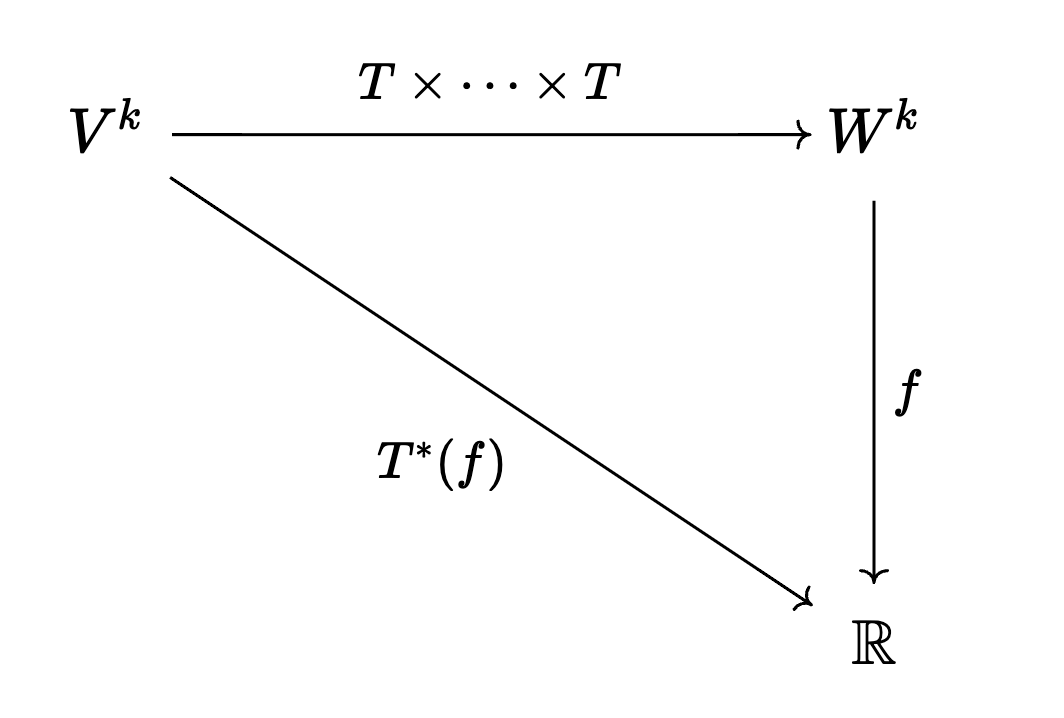
\includegraphics[scale=0.3]{images/Screenshot 2023-02-28 at 14.35.26.png}
    \end{figure}
\end{itemize}

\begin{theorem}[Properties of dual transformation]
    Let $T\in \mathcal{L}(V,W)$ be a linear transformation. Let $T^*$ be the dual transformation. Then
    \begin{enumerate}
        \item $T^*$ is linear.
        \item $T^*(f\otimes g)=T^*f \otimes T^*g$
        \item If $S\in \mathcal{L}(W,X)$, then $(S\circ T)^*(f)=T^*(S^*(f))$
        \begin{figure}[H]
            \centering
            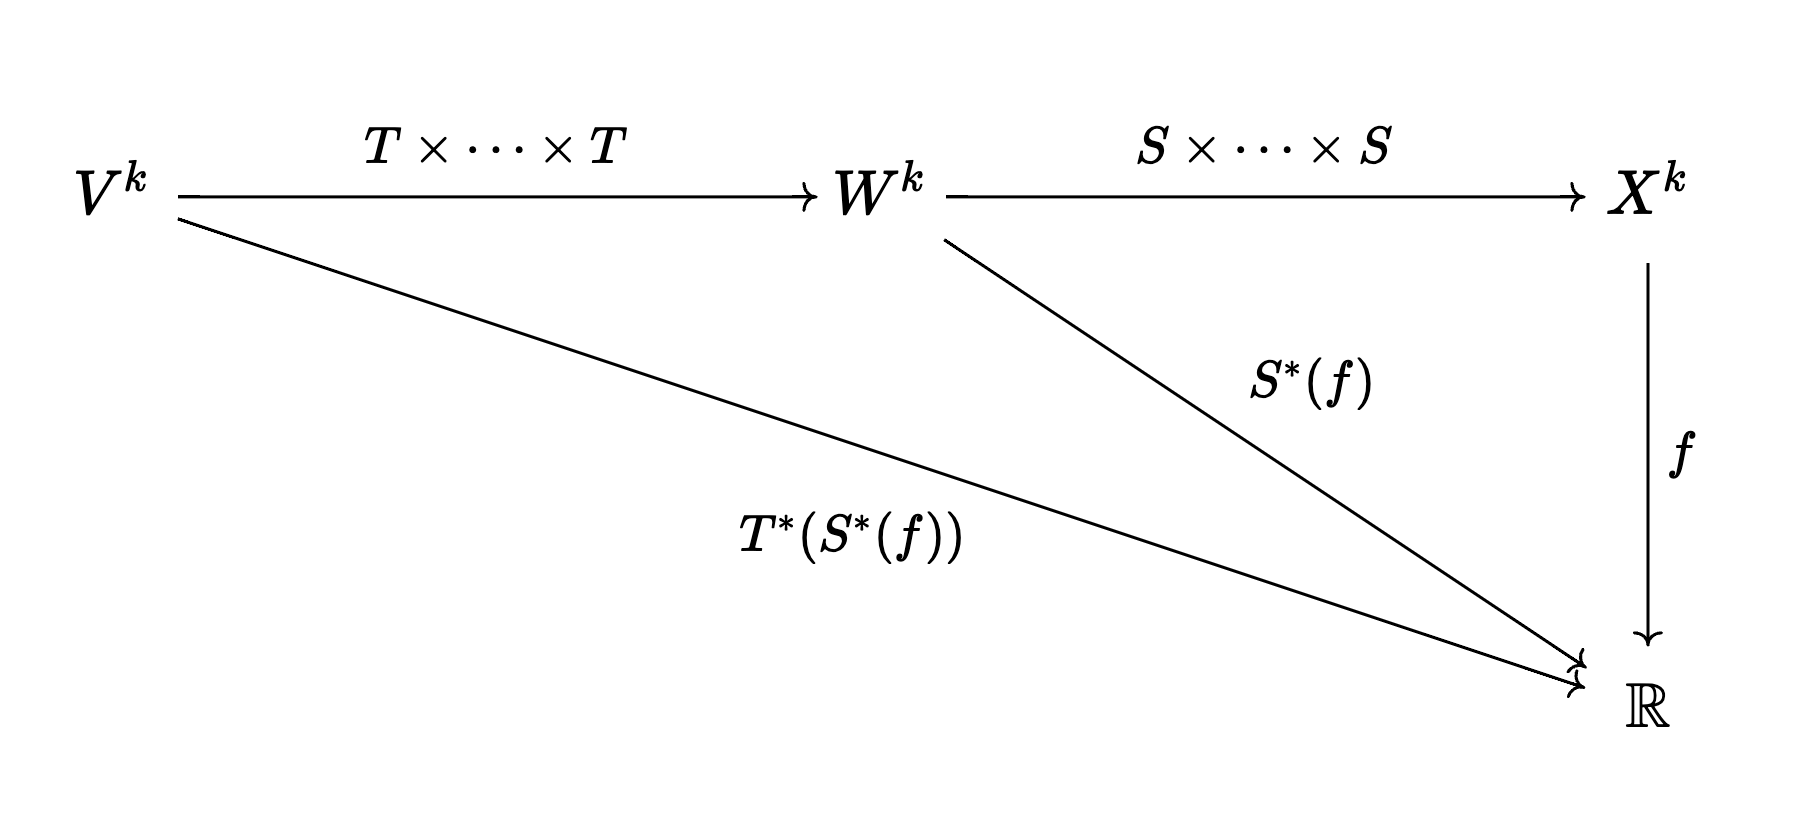
\includegraphics[scale=0.3]{images/Screenshot 2023-02-28 at 14.52.28.png}
        \end{figure}
        \begin{figure}[H]
            \centering
            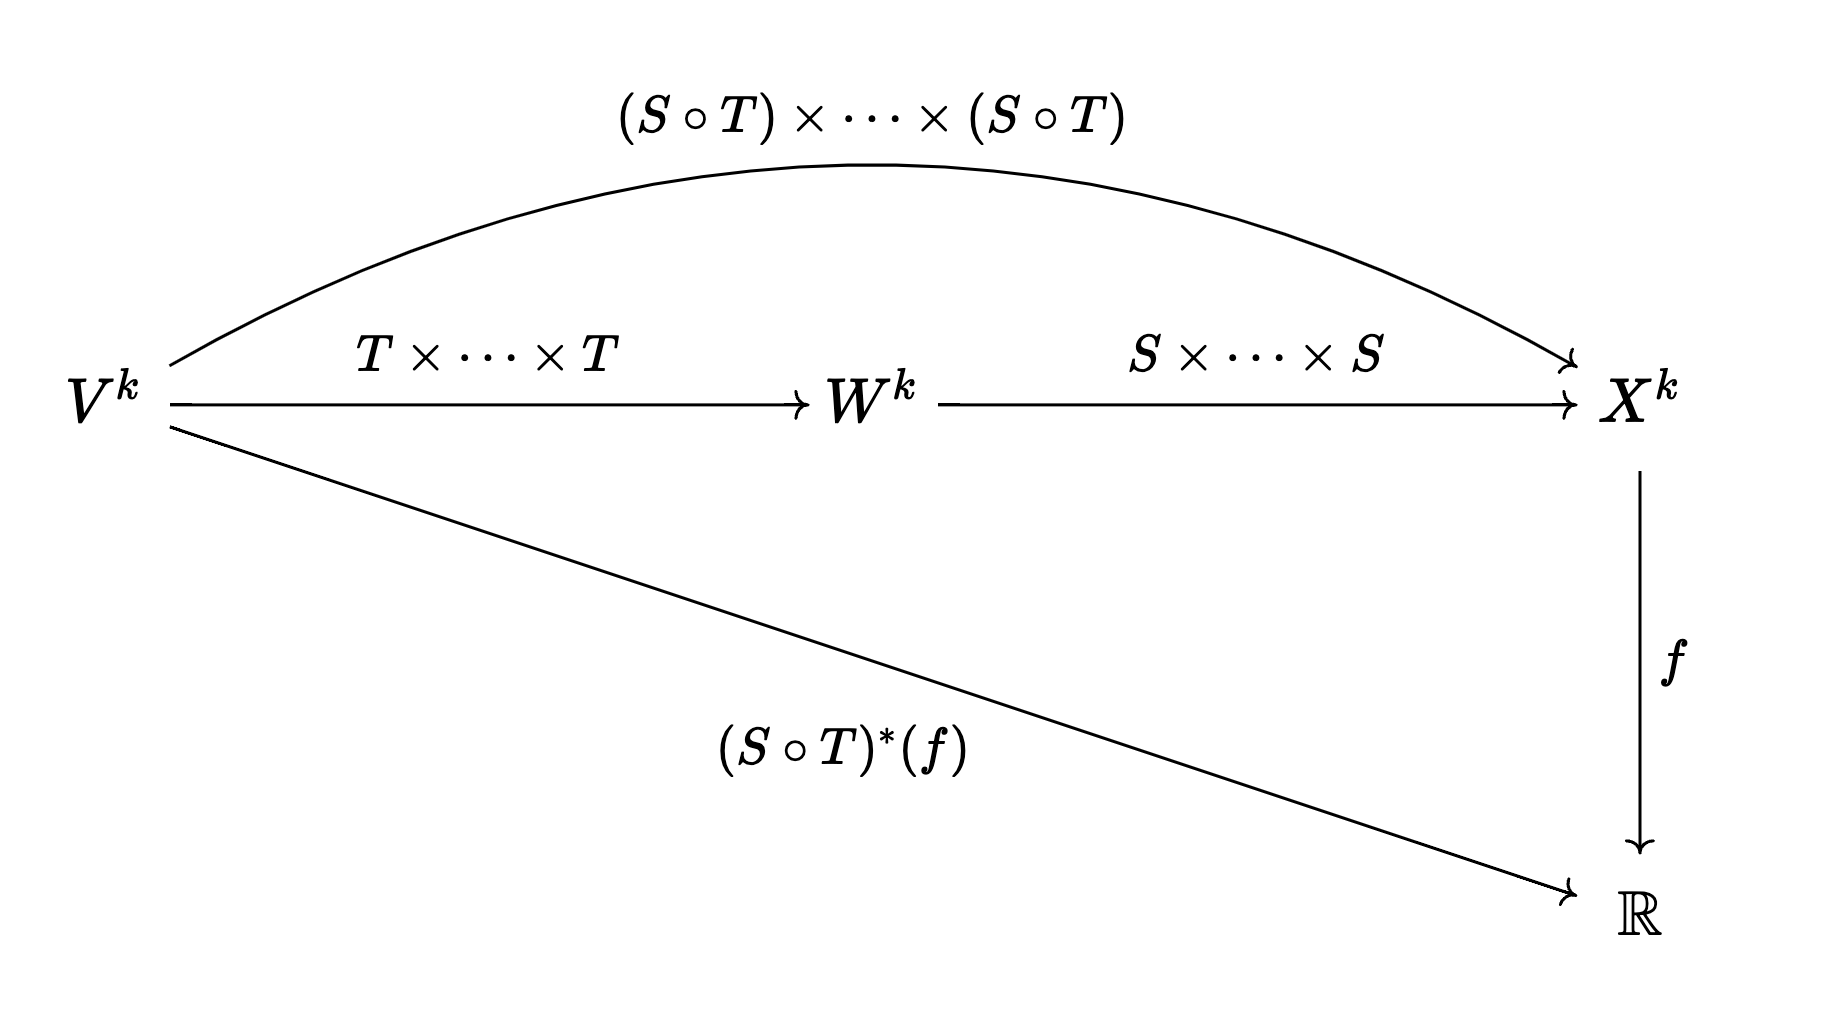
\includegraphics[scale=0.3]{images/Screenshot 2023-02-28 at 14.52.38.png}
        \end{figure}
    \end{enumerate}
\end{theorem}

\section{Alternating Tensors}

\begin{definition}
    Given the set $\{1,\cdots,k\}$ with $k\geq 2$. A \underline{permutation} is a bijective function 
    $$\sigma:\{1,\cdots,k\}\longrightarrow\{1,\cdots,k\}$$
    We denote the set of all such permutations by $S_k$. The set $S_k$ forms a group, called the \underline{symmetric group} on the set $\{1,\cdots,k\}$.
\end{definition}
\noindent\textbf{Remark}:
\begin{itemize}
    \item $S_k$ is a group because if $\sigma$ and $\tau$ are elements of $S_k$, so are $\sigma\circ \tau$ and $\sigma^{-1}$.
    \item The symmetric group $S_k$ has $k!$ elements.
\end{itemize}

\begin{definition}
    Given $1\leq i <k$, let $e_i$ be the element of $S_k$ defined by setting 
    $$e_i(i)=i+1$$
    $$e_i(i+1)=i$$
    $$e_i(j)=j \text{ for }j\neq i,i+1$$
    The permutation $e_i$ is called the \underline{elementary permutation}.
\end{definition}
\noindent\textbf{Remark}:
\begin{itemize}
    \item Consider $e_i$ as an action on the set $\{1,\cdots,k\}$. It means we flip the elements $i,i+1$ and let others be fixed.
    \item $e_i\circ e_i=e$ where $e$ is the identity permutation. This is because we flip $i,i+1$ twice and let others be fixed.
\end{itemize}

\begin{lemma}
    If $\sigma\in S_k$, then $\sigma$ equals a composite of elementary permutations.
\end{lemma}

\begin{definition}
    Let $\sigma\in S_k$. Consider the set of all pairs of integers $i,j$ from the set $\{1,\cdots,k\}$ for which $i<j$ and $\sigma(i)>\sigma(j)$. Each such pair is called an inversion in $\sigma$.
    \begin{itemize}
        \item We define the \underline{sign} of $\sigma$ to be the number $-1$ if the number of inversions in $\sigma$ is odd.
        $$sgn(\sigma)=-1$$
        In this case, we call $\sigma$ an \underline{odd permutation}.
        \item We define the \underline{sign} of $\sigma$ to be the number $1$ if the number of inversions in $\sigma$ is even.
        $$sgn(\sigma)=1$$
        In this case, we call $\sigma$ an \underline{even permutation}.
    \end{itemize}
\end{definition}

\begin{lemma}
    Let $\sigma,\tau\in S_k$.
    \begin{enumerate}
        \item If $\sigma$ equals to a composite of $m$ elementary permutations, then $$sgn(\sigma)=(-1)^m$$
        Sometimes we will use this to define $sgn(\sigma)$.
        \item $sgn(\sigma\circ \tau)=sgn(\sigma)sgn(\tau)$
        \item $sgn(\sigma^{-1})=sgn(\sigma)$
        \item Let $p\neq q$, if $\tau$ is the permutation that exchanges $p$ and $q$ and leaves all other integers fixed, then $sgn(\tau)=-1$.
    \end{enumerate}
\end{lemma}

\begin{definition}
    Let $f\in\mathcal{L}^k(V)$. Let $\sigma\in S_k$. We define $f^{\sigma}$ by the equation 
    $$f^{\sigma}(v_1,\cdots,v_k)=f(v_{\sigma(1)},\cdots,v_{\sigma(k)})$$
    It means we permutes the vectors $(v_1,\cdots,v_k)$ to $(v_{\sigma(1)},\cdots,v_{\sigma(k)})$ and then apply $f$. Because $f$ is linear in each of variables, so is $f^{\sigma}$, so $f^{\sigma}$ is a k-tensor on $V$. 
    \begin{itemize}
        \item The tensor $f$ is said to be \underline{symmetric} if $$f^{e_i}=f$$ 
        $$f(v_1,\cdots,v_{i+1},v_i,\cdots,v_k)=f(v_1,\cdots,v_i,v_{i+1},\cdots,v_k)$$
        for each elementary permutation $e_i$.
        \item The tensor $f$ is said to be \underline{alternating} if $$f^{e_i}=-f$$ 
        $$f(v_1,\cdots,v_{i+1},v_i,\cdots,v_k)=-f(v_1,\cdots,v_i,v_{i+1},\cdots,v_k)$$
        for each elementary permutation $e_i$.
    \end{itemize}
\end{definition}

\begin{definition}
    Let $V$ be a vector space, we denote the set of alternating k-tensors on $V$ by $\mathcal{A}^k(V)$. It is easy to check that the sum of two alternating tensors is alternating , and that so is a scalar multiple of an alternating tensor. 
    Then $$\mathcal{A}^k(V)\subset \mathcal{L}^k(V)$$
    $\mathcal{A}^k(V)$ is a linear subspace of the vector space $\mathcal{L}^k(V)$. 
    The condition that a 1-tensor be alternating is vacuously true. Therefore we make the convention that $$\mathcal{A}^1(V)=\mathcal{L}^1(V)$$
\end{definition}

\noindent\textbf{Example}: Alternating tensors.
\begin{itemize}
    \item Alternating 1-tensors.
    \begin{enumerate}
        \item $\mathcal{A}^1(V)=\mathcal{L}^1(V)$ by our definition.
    \end{enumerate}
    \item Alternating 2-tensors.
    \begin{enumerate}
        \item Given vector space $V$ with basis $\{a_1,\cdots,a_n\}$. Consider elementary 2-tensors $\{\phi_{i,j}\}$. Define 
        $$f(v,w)=\phi_{i,j}(v,w)-\phi_{j,i}(v,w)$$
        We can verify that 
        \begin{equation*}
            \begin{split}
                f(w,v) &= \phi_{i,j}(w,v)-\phi_{j,i}(w,v)\\
                &= \phi_i(w)\phi_j(v)-\phi_j(w)\phi_i(v)\\
                &= -(\phi_i(v)\phi_j(w)-\phi_j(v)\phi_i(w))\\
                &= -f(v,w)
            \end{split}
        \end{equation*}
    \end{enumerate}
    \item Alternating n-tensors.
    \begin{enumerate}
        \item Given the vector space $V=\R^n$ with usual basis. Given $n$ vectors $v_1,\cdots,v_n$. Define
        $$f(v_1,\cdots,v_n)=\det(\begin{bmatrix}
            v_1 & \cdots & v_n
        \end{bmatrix})$$
        In MAT240, we learnt that the determinant is skew-symmetry. 
        $$\det(\begin{bmatrix}
            v_1 & \cdots & v_i & \cdots & v_j & \cdots & v_n
        \end{bmatrix})=-\det(\begin{bmatrix}
            v_1 & \cdots & v_j & \cdots & v_i & \cdots & v_n
        \end{bmatrix})$$
        Therefore, $f$ is an alternating n-tensor on $V$.
    \end{enumerate}
\end{itemize}

\begin{lemma}
    Let $f$ be a k-tensor on $V$. Let $\sigma,\tau\in S_k$.
    \begin{enumerate}
        \item The transformation $f\longrightarrow f^{\sigma}$ is an element of $\mathcal{L}(\mathcal{L}^k(V))$. 
        It has the property that for all $\sigma,\tau$, $$(f^{\sigma})^{\tau}=f^{\tau\circ\sigma}$$
        \item The tensor $f$ is alternating if and only if $$f^{\sigma}=sgn(\sigma)\cdot f$$ for all $\sigma\in S_k$.\\
        It follows trivially that if $f$ is alternating and if $v_p=v_q$ with $p\neq q$, then $$f(v_1,\cdots,v_k)=0$$
    \end{enumerate}
\end{lemma}

\begin{lemma}
    Given vector space $V$ with basis $\{a_1,\cdots,a_n\}$. Let $f,g\in \mathcal{L}^k(V)$. If for every ascending k-tuple $I=(i_1,\cdots,i_k)$ for the set $\{1,\cdots,n\}$ we have $$f(a_{i_1},\cdots,a_{i_k})=g(a_{i_1},\cdots,a_{i_k})$$
    Then we have $f=g$.
\end{lemma}

\begin{theorem}
    Given vector space $V$ with basis $\{a_1,\cdots,a_n\}$. Let $I=(i_1,\cdots,i_k)$ be an ascending k-tuple from the set $\{1,\cdots,n\}$. There is a unique alternating k-tensor $\psi_I$ n $V$ such that for every ascending k-tuple $J=(j_1,\cdots,j_k)$ from the set $\{1,\cdots,n\}$, 
    \begin{equation*}
        \psi_I(a_{j_1},\cdots,a_{j_k})=\begin{cases}
            0 \text{ if }I\neq J\\
            1 \text{ if }I =J
        \end{cases}
    \end{equation*}
    The tensors $\{\psi_I\}$ form a basis for $\mathcal{A}^k(V)$. The tensors $\psi_I$ in fact satisfies the formula 
    $$\psi_I=\sum_{\sigma\in S_k}sgn(\sigma)(\phi_I)^{\sigma}$$
\end{theorem}

\begin{definition}
    The tensors $\{\psi_I\}$ are called the \underline{elementary alternating k-tensors} on $V$ corresponding to the basis $\{a_1,\cdots,a_n\}$.
\end{definition}
\noindent\textbf{Remark}:
\begin{itemize}
    \item The theorem above shows that given basis $\{a_1,\cdots,a_n\}$ for $V$, an arbitrary alternating k-tensor $f$ can be written uniquely in the form $$f=\sum_{[J]}d_J\psi_J$$
    The numbers $d_J$ are called \underline{components} of $f$ relative to the basis $\{\psi_J\}$.
    \item For $k=1$, $dim(\mathcal{A}^1(V))=dim(\mathcal{L}^1(V))=dim(V^*)=dim(V)=n$.\\
    For $1<k\leq n$. Given $\{1,\cdots,n\}$, we have ${n \choose k}$ numbers of subsets of $k$ elements. For each subset, there is exactly one corresponding ascending k-tuple. Therefore we have ${n \choose k}$ many elementary alternating k-tensors.
    Thus $$dim(\mathcal{A}^k(V))={n \choose k}=\frac{n!}{k!(n-k)!}$$
\end{itemize}

\begin{theorem}
    Let $T:V\longrightarrow W$ be a linear transformation. If $f$ is an alternating tensor on $W$, then $T^*(f)$ is an alternating tensor on $V$.
\end{theorem}

\begin{theorem}[Equivalent definition of determinant]
    Let $\{e_1,\cdots,e_n\}$ be the usual basis for $\R^n$. Let $\{\phi_i\}$ be the dual basis for $\mathcal{L}^1(V)=V^*$. 
    \begin{equation*}
        \begin{split}
            \det([v_1,\cdots,v_n])&=\psi_{(1,2,\cdots,n)}(v_1,\cdots,v_n)\\
            &= \sum_{\sigma\in S_n}sgn(\sigma)\phi_I(v_{\sigma(1)},\cdots,v_{\sigma(n)})\\
            &= \sum_{\sigma\in S_n}sgn(\sigma)v_{1,\sigma(1)}\cdots v_{n,\sigma(n)}
        \end{split}
    \end{equation*}
\end{theorem}
\noindent\textbf{Remark}:
\begin{itemize}
    \item This is the definition of determinant we learnt in MAT240. 
    \item In chapter1 of the text book, the determinant of n by n matrix is defined to be a function that satisfies three axioms. This theorem gives us a way to express that abstract function explicitly.
\end{itemize}

\begin{theorem}
    Let $\psi_I$ be an elementary alternating tensor on $\R^n$ corresponding to the usual basis. Given vectors $x_1,\cdots,x_k$ of $\R^n$. Let $X$ be the matrix $X=[x_1 \cdots x_k]$. Then 
    $$\psi_I(x_1,\cdots,x_k)=\det(X_I)$$
    where $X_I$ denotes the matrix whose successive rows are rows $i_1,\cdots,i_k$ of $X$.
\end{theorem}
\noindent\textbf{Example}:
\begin{itemize}
    \item Consider the space $\mathcal{A}^3(\R^4)$. The elementary alternating 3-tensors on $\R^4$, corresponding to the ususal basis are the functions 
    \begin{equation*}
        \psi_{(i,j,k)}(x,y,z)= \det(\begin{bmatrix}
            x_i & y_i & z_i\\
            x_j & y_j & z_j\\
            x_k & y_k & z_k
        \end{bmatrix})
    \end{equation*}
    where $(i,j,k)$ is ascending, so it equals $(1,2,3)$ or $(1,2,4)$ or $(1,3,4)$ or $(2,3,4)$. 
    The general elements of $\mathcal{A}^3(\R^4)$ is a linear combination of these four functions.
\end{itemize}

\section{The Wedge Product}

\noindent \textbf{Motivation}:
\begin{itemize}
    \item Recall the tensor product $$\otimes:\mathcal{L}^k(V)\times\mathcal{L}^l(V)\longrightarrow\mathcal{L}^{k+l}(V)$$ If $f\in\mathcal{A}^k(V)$ and $g\in\mathcal{A}^l(V)$, then the tensor product cannot guarantee that $f\otimes g$ be an element of $\mathcal{A}^{k+l}(V)$. In fact, $f\otimes g$ is almost never alternating. 
    \item Since we want to focus on the space $\mathcal{A}^n(V)$. It is our desire to make an operation $$\wedge : \mathcal{A}^k(V)\times \mathcal{A}^l(V)\longrightarrow\mathcal{A}^{k+l}(V)$$
\end{itemize}


\begin{definition}
    Given a k-tensor $f\in \mathcal{L}^k(V)$. We define the \underline{alternating operator} by 
    $$Alt(f)=\sum_{\sigma\in S_k}sgn(\sigma)f^{\sigma}$$ 
\end{definition}
\noindent\textbf{Remark}:
\begin{itemize}
    \item It follows trivially that $$\psi_I=Alt(\phi_I)$$
    \item The alternating operator is an important tool in the study of differential forms and exterior algebra, and it plays a key role in many areas of mathematics and physics, including differential geometry, topology, and quantum mechanics.
\end{itemize}

\begin{theorem}[Properties of alternating operator]
    Given a k-tensor $f\in \mathcal{L}^k(V)$. Let $Alt$ be the alternating operator, then 
    \begin{enumerate}
        \item $Alt$ is linear.
        \item $Alt(f)\in \mathcal{A}^k(V)$
        \item If $f\in \mathcal{A}^k(V)$, then $Alt(f)=(k!)f$.
    \end{enumerate}
\end{theorem}

\begin{corollary}
    The alternating operator is a linear map. $$Alt:\mathcal{L}^k(V)\longrightarrow\mathcal{A}^k(V)$$
\end{corollary}

\begin{lemma}
    Given $f\in\mathcal{L}^k(V)$ and $g\in\mathcal{L}^l(V)$, then we have $$Alt(f\otimes g)=(-1)^{kl}Alt(g\otimes f)$$
\end{lemma}

\noindent\textbf{Remark}:
\begin{itemize}
    \item Later, we will use the alternating operator $Alt$ to define the wedge product. And the lemma above is useful to prove the properties of $\wedge$.
    \item For now, we can use $Alt$ to learn the structure of the vector space $\mathcal{L}^k(V)$. In other words, to decompose the vector space $\mathcal{A}^k(V)$.
\end{itemize}

\begin{definition}
    A k-tensor $f\in\mathcal{L}^k(V)$ is \underline{decomposible} if $$f=l_1\otimes \cdots \otimes l_k$$
    where $l_i\in \mathcal{L}^1(V)=V^*$ are all 1-tensors. The decomposible k-tensor $f$ is \underline{redundant} if for some index $i$, we have $l_i=l_{i+1}$. We define the set $\mathcal{I}^k(V)$ as 
    $$\mathcal{I}^k(V)=\text{ linear span }\{\text{ redundant k-tensors }\} $$
    Note that for $k=1$ the notion of redundant does not really make sense, a single 1-tensor cannot be written as the product of two 1-tensors, so we make the following definition $$\mathcal{I}^1(V)=\{0\}$$
\end{definition}

\begin{lemma}\
    Let $f\in\mathcal{L}^k(V)$ and $\sigma\in S_k$, then there exisis $g\in \mathcal{I}^k(V)$ such that $$f^{\sigma}=sgn(\sigma)f+g$$
\end{lemma}
\noindent\textbf{Remark}:
\begin{itemize}
    \item In the proof of the theorem, we can assume without loss of generality that $f$ is decomposable, because any tensor can be decomposed into a sum of decomposable tensors.
\end{itemize}


\begin{corollary}
    For any $f\in\mathcal{L}^k(V)$, there exisis $g\in\mathcal{I}^k(V)$ such that $$Alt(f)=(k!)f+g$$
\end{corollary}

\begin{theorem}
    Let $Alt$ be the alternating operator on k-tensors on $V$, then $$\ker(Alt)=\mathcal{I}^k(V)$$
\end{theorem}

\begin{corollary}
    $$\mathcal{L}^k(V)=\mathcal{A}^k(V) \oplus \mathcal{I}^k(V)$$
\end{corollary}

\begin{definition}
    The \underline{k-fold exterior product} of $V$ is defined as the quotient of the vector space $\mathcal{L}^k(V)$ and the subspace $\mathcal{I}^k(V)$. $$\Lambda^k(V^*)=\mathcal{L}^k(V)/\mathcal{I}^k(V)$$
\end{definition}

\noindent\textbf{Remark}:
\begin{itemize}
    \item If $V$ is finite dimensional, we have a natrual isomorphic
    $$\Lambda^k(V^*)\cong \mathcal{A}^k(V)$$
    Some books will abuse the notation.
\end{itemize}

\begin{definition}
    Let $f\in\mathcal{L}^k(V)$ and $g\in \mathcal{L}^l(V)$. Then we define the \underline{wedge product} of $f$ and $g$ as $$f \wedge g=\frac{1}{k!l!}Alt(f\otimes g)$$
\end{definition}

\begin{lemma}
    Let $f$ be an arbitrary tensor and $h$ be an alternating m-tensor, then $$Alt(f)\wedge h=\frac{1}{m!}Alt(f\otimes h)$$
\end{lemma}

\begin{theorem}[Properties of wedge product]
    Let $V$ be a vector space with basis $\{a_1,\cdots,a_n\}$. Let $f\in\mathcal{A}^k(V)$ and $g\in\mathcal{A}^l(V)$, then we have 
    \begin{enumerate}
        \item (Associativity) $$f\wedge (g\wedge h)=(f\wedge g)\wedge h$$
        \item (Homogeneity) $$(cf)\wedge g=c(f\wedge g)=f\wedge(cg)$$
        \item (Distributivity) If $f$ and $g$ have the same order, $k=l$, then $$(f+g)\wedge h=f\wedge h + g\wedge h$$ $$h\wedge(f+g)=h\wedge f +h\wedge g$$
        \item (Anti-commutativity) $$g\wedge f=(-1)^{kl}f\wedge g$$
        \item Let $\{\phi_i\}$ be the dual basis. Let $\{\psi_I\}$ be the elementary alternating tensors where $I=(i_1,\cdots,i_k)$ be an ascending k-tuple, then $$\psi_I=\phi_{i_1}\wedge \cdots \wedge\phi_{i_k}$$
    \end{enumerate}
\end{theorem}
\noindent\textbf{Remark}:
\begin{itemize}
    \item These properties characterize the wedge product uniquely for finite dimension $V$. This theorem can be used as an equivalent definition of the wedge product.
\end{itemize}

\begin{theorem}
    Let $T\in\mathcal{L}(V,W)$, let $f\in\mathcal{A}^k(W)$ and $g\in\mathcal{A}^l(W)$. We have the dual transformation $T^*\in\mathcal{L}(\mathcal{L}^{k+l}(W),\mathcal{L}^{k+l}(V))$ then $$T^*(f\wedge g)=T^*(f)\wedge T^*(g)$$
\end{theorem}

\section{Tangent Vector Field}

\begin{definition}
    Given $x\in \R^n$, we define a \underline{tangent vector} to $\R^n$ at $x$ to be a pair $(x;v)$, where $v\in \R^n$. We define the \underline{tangent space} as $$\mathcal{T}_x(\R^n)=\{(x;v): v\in \R^n\}$$
    The space $\mathcal{T}_x(\R^n)$ is a vector space if we define 
    \begin{enumerate}
        \item (Vector addition) $$(x;v)+(x;w)=(x;v+w)$$
        \item (Scalar multiplication) $$c(x;v)=(x;cv)$$
    \end{enumerate}
\end{definition}

\noindent\textbf{Remark}:
\begin{itemize}
    \item It is easy to see that $$\mathcal{T}_x(\R^n)=\{x\}\times \R^n \cong \R^n$$
    Via this identification, the vector space structure on $\R^n$ gives a vector space structure on $\mathcal{T}_x(\R^n)$.
    \item Intuitively, we can think $v$ as an arrow centered at the point $x$.
\end{itemize}

\begin{definition}
    Let $(a,b)\subset \R$. Let $\gamma:(a,b)\subset \R\longrightarrow \R^n$ be a map of class $C^r$. The image of $\gamma$ is a parametrized-curve. 
    We define the \underline{velocity vector} of $\gamma$ corresponding to the parameter value $t$ as $$(\gamma(t);D\gamma(t))$$
\end{definition}
\noindent\textbf{Remark}:
\begin{itemize}
    \item Consider the case $\gamma:(a,b)\longrightarrow\R^3$. Let $$\gamma(t)=(x(t),y(t),z(t))$$
    \begin{equation*}
        D\gamma(t)=\begin{bmatrix}
            x'(t)\\
            y'(t)\\
            z'(t)
        \end{bmatrix}
    \end{equation*}
    $\gamma(t)$ gives us the position at time $t$ and $D\gamma(t)$ tells us the velocity at $\gamma(t)$.
\end{itemize}

\begin{definition}
    Let $A$ be open in $\R^k$ or $\HH^k$. Let $\alpha:A\longrightarrow\R^n$ be of class $C^r$. 
    Let $x\in A$ and let $p=\alpha(x)$. We define a linear transformation $$\alpha_*:\mathcal{T}_x(\R^k)\longrightarrow\mathcal{T}_p(\R^n)$$ by the equation 
    $$\alpha_*(x;v)=(p;D\alpha(x)\cdot v)$$
    The linear transformation $\alpha_*$ is said to be \underline{induced} by the differentiable map $\alpha$.
\end{definition}
\noindent\textbf{Remark}:
\begin{itemize}
    \item The definition of $\alpha_*$ can be shown in the following diagram.
    \begin{figure}[H]
        \centering
        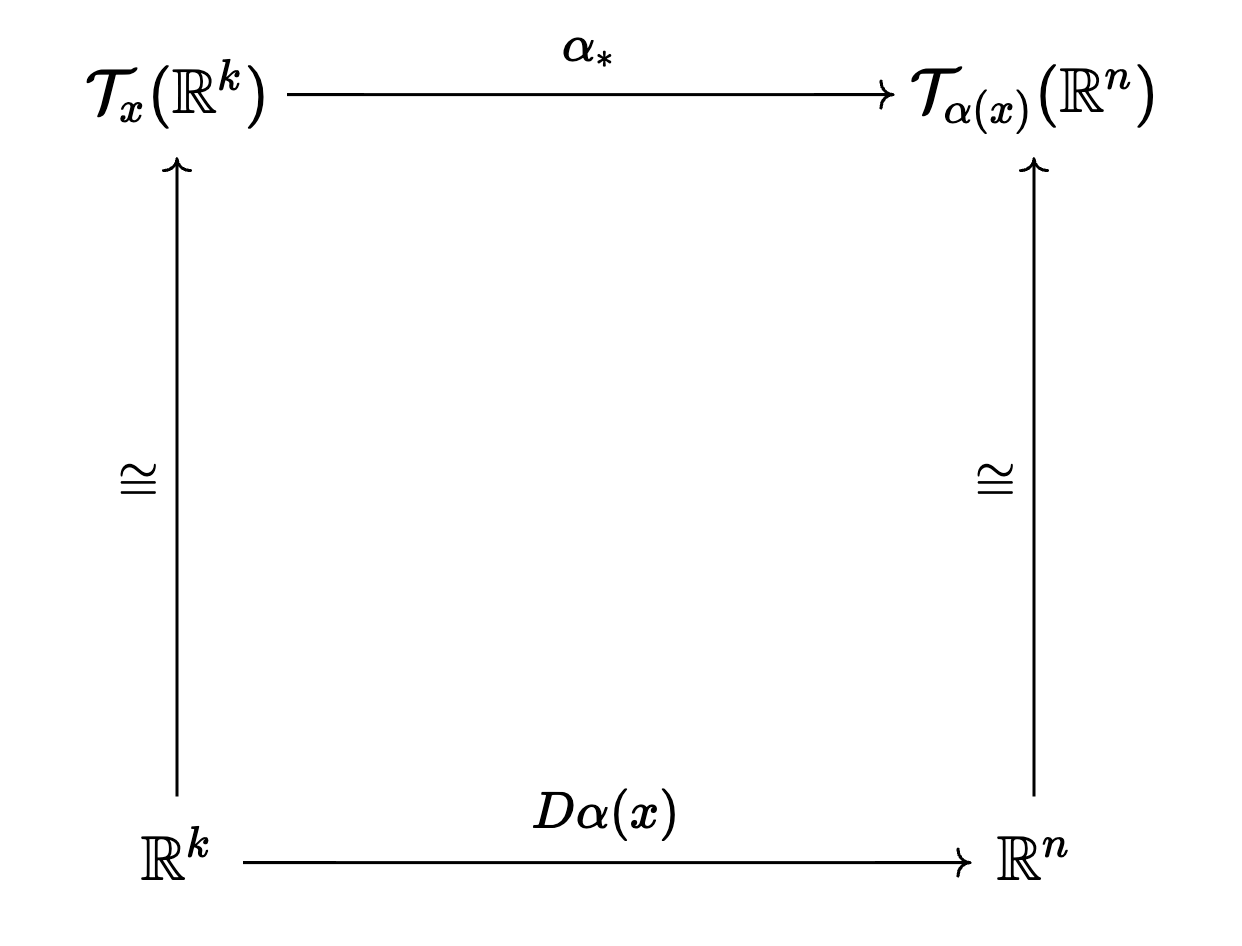
\includegraphics[scale=0.3]{images/Screenshot 2023-03-09 at 19.37.08.png}
    \end{figure}
    \item Sometimes we write $\alpha_*$ as $d\alpha_x$, this tells us that we are actually defining the differential(vector-valued differential form) on the tangent space.
    \item Consider the case $\alpha:A\subset\R^2\longrightarrow\R^3$ that we can visualize. Let $$\gamma(t)=\alpha(x+tv)$$ be the parametrized-curve on the image $\alpha(A)$ in $\R^3$.
    \begin{figure}[H]
        \centering
        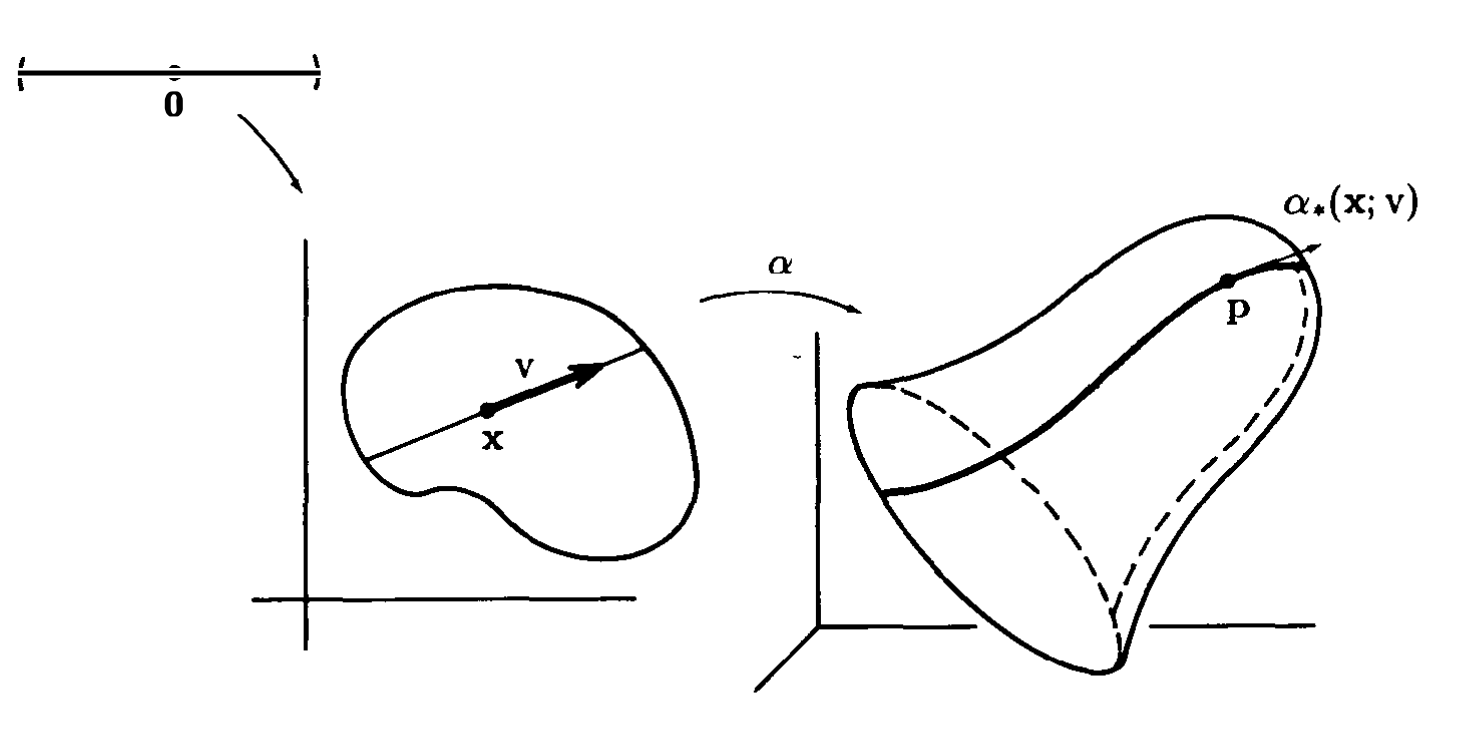
\includegraphics[scale=0.45]{images/Screenshot 2023-03-09 at 19.48.13.png}
    \end{figure}
    We start at the point $p=\alpha(x)$, after time $t$, we are at the position $\gamma(t)=\alpha(x+tv)$. 
    The velocity can be computed by the chain rule
    \begin{equation*}
        D\gamma(t)=D\alpha(x+tv)\cdot v
    \end{equation*}
    The induced transformation is $$\alpha_*(x;v)=(\alpha(x);D\alpha(x)\cdot v)$$
    which is equal to the velocity vector of $\gamma(t)$ at $t=0$.
\end{itemize}

\begin{lemma}
    Let $A$ be open in $\R^k$ or $\HH^k$. Let $\alpha:A\longrightarrow\R^m$ be of class $C^r$. 
    Let $B$ be open in $\R^k$ or $\HH^k$ containing $\alpha(A)$. Let $\beta:B\longrightarrow\R^n$ be of class $C^r$. Then $$(\beta\circ \alpha)_*=\beta_*\circ \alpha_*$$
\end{lemma}
\noindent\textbf{Remark}:
\begin{itemize}
    \item The proof is trivial, consider the following diagram.
    \begin{figure}[H]
        \centering
        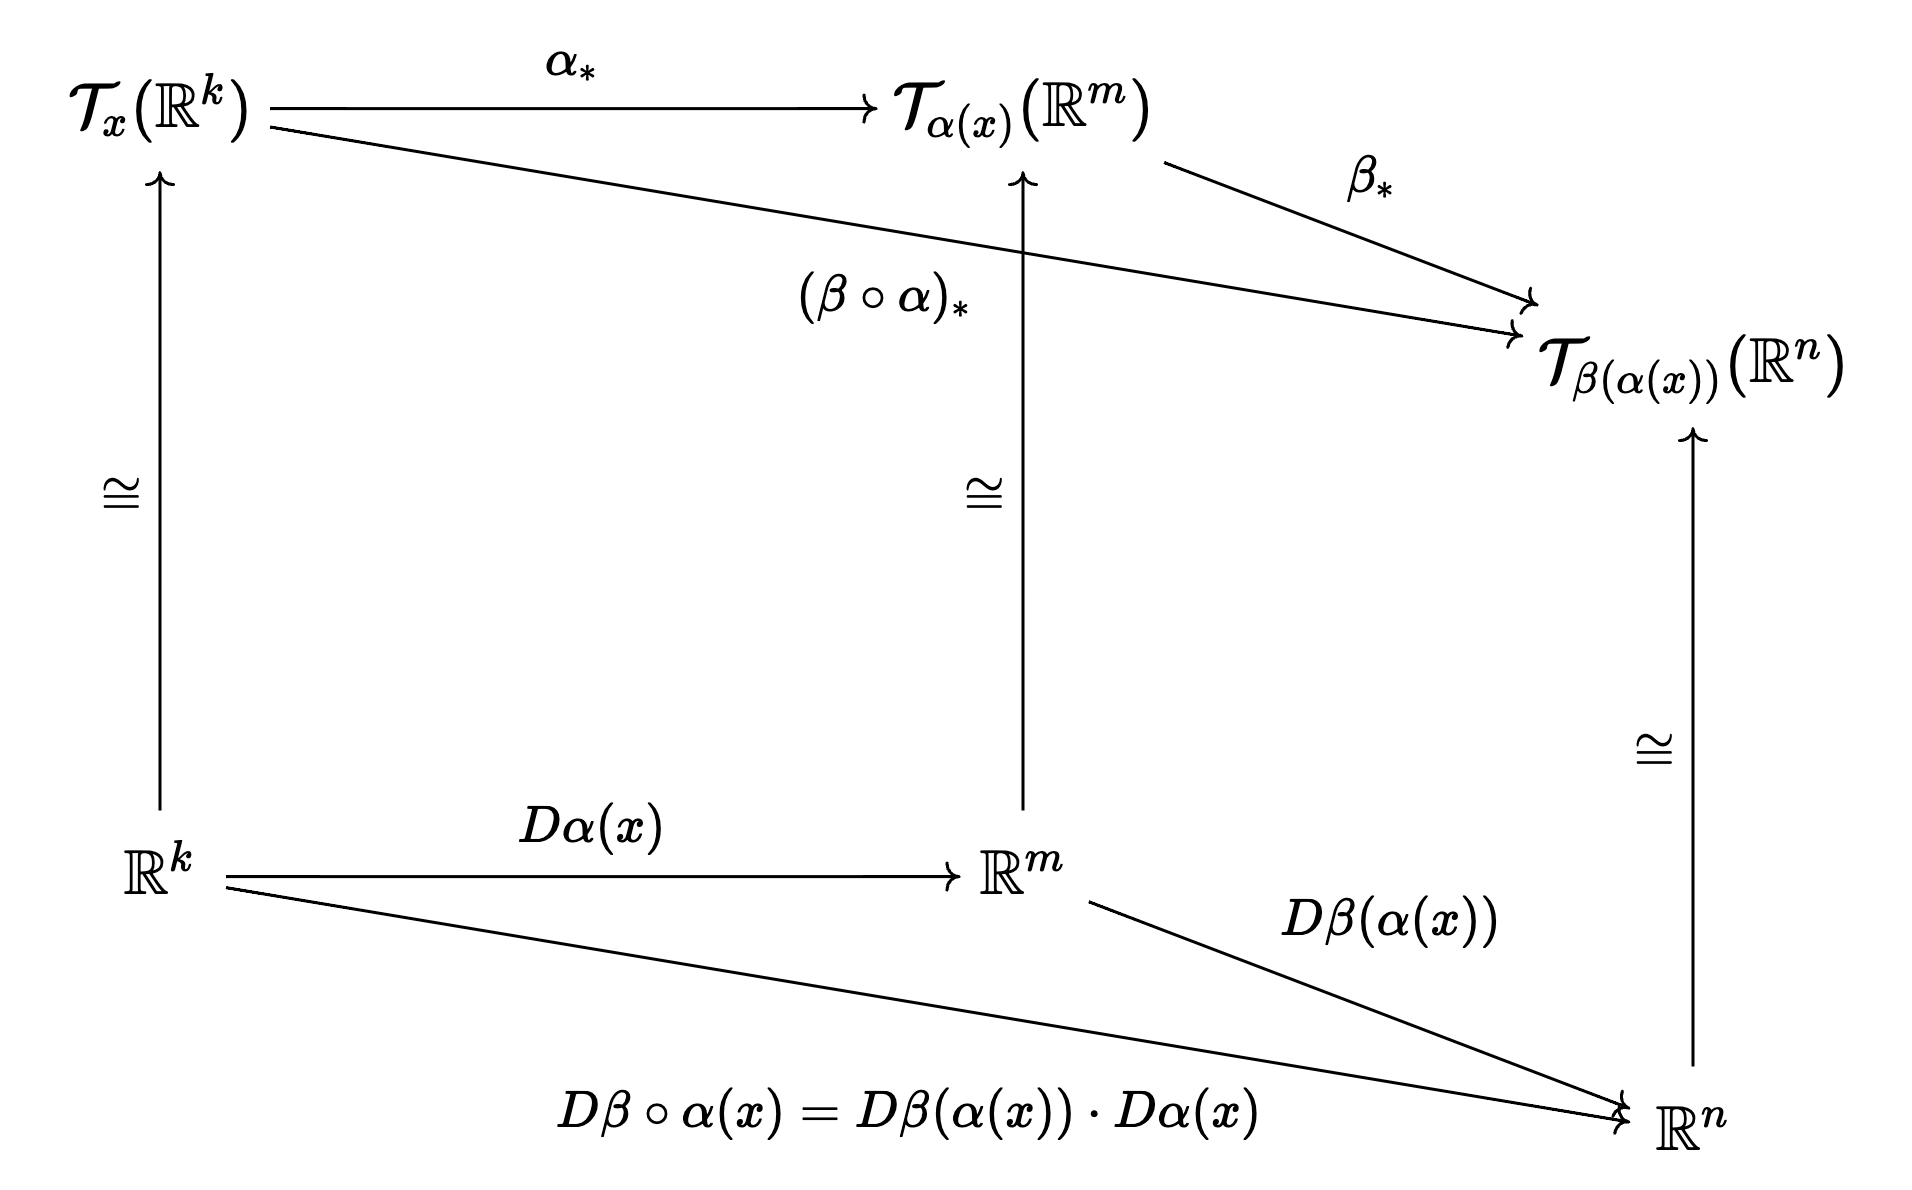
\includegraphics[scale=0.3]{images/Screenshot 2023-03-09 at 20.12.07.png}
    \end{figure}
\end{itemize}

\begin{definition}
    Let $A$ be an open set in $\R^n$, the \underline{tangent vector field} in $A$ is a continuous function $F$
    such that $$\forall x\in A. F(x)=(x;f(x))$$ where $f:A\longrightarrow\R^n$. If $F$ is of class $C^r$, we say that it is a tangent vector field of class $C^r$.
\end{definition}
\noindent\textbf{Remark}:
\begin{itemize}
    \item The tangent field $F$ tells us that if we have a function $f:A\subset\R^n\longrightarrow\R^n$. Then for any vector $x\in A$, we can assign a tangent vector $(x;f(x))$.
\end{itemize}

\begin{definition}
    Let $M$ be a k-manifold of class $C^r$ in $\R^n$. Let $p\in M$, choose a coordinate patch $\alpha:U\longrightarrow V$ about $p$ where $U$ is open in $\R^k$ or $\HH^k$. 
    Let $x$ be the point in $U$ such that $\alpha(x)=p$. The \underline{tangent space to $M$ at $p$} is defined as $$\mathcal{T}_p(M)=\{\alpha_*(x;v):v\in \R^k\}\subset\mathcal{T}_p(\R^n)$$
\end{definition}
\noindent\textbf{Remark}:
\begin{itemize}
    \item It is not hard to show that $\mathcal{T}_p(M)$ is a linear subspace of $\mathcal{T}_p(\R^n)$. Let $\{e_1,\cdots,e_k\}$ be the basis of $\R^k$. Then the space $\mathcal{T}_p(M)$ is spanned by the vectors $$\{(p;D\alpha(x)\cdot e_j)\}=\{(p;\frac{\partial \alpha}{\partial x_j})\}$$
    The follwing graph gives the intuition.
    \begin{figure}[H]
        \centering
        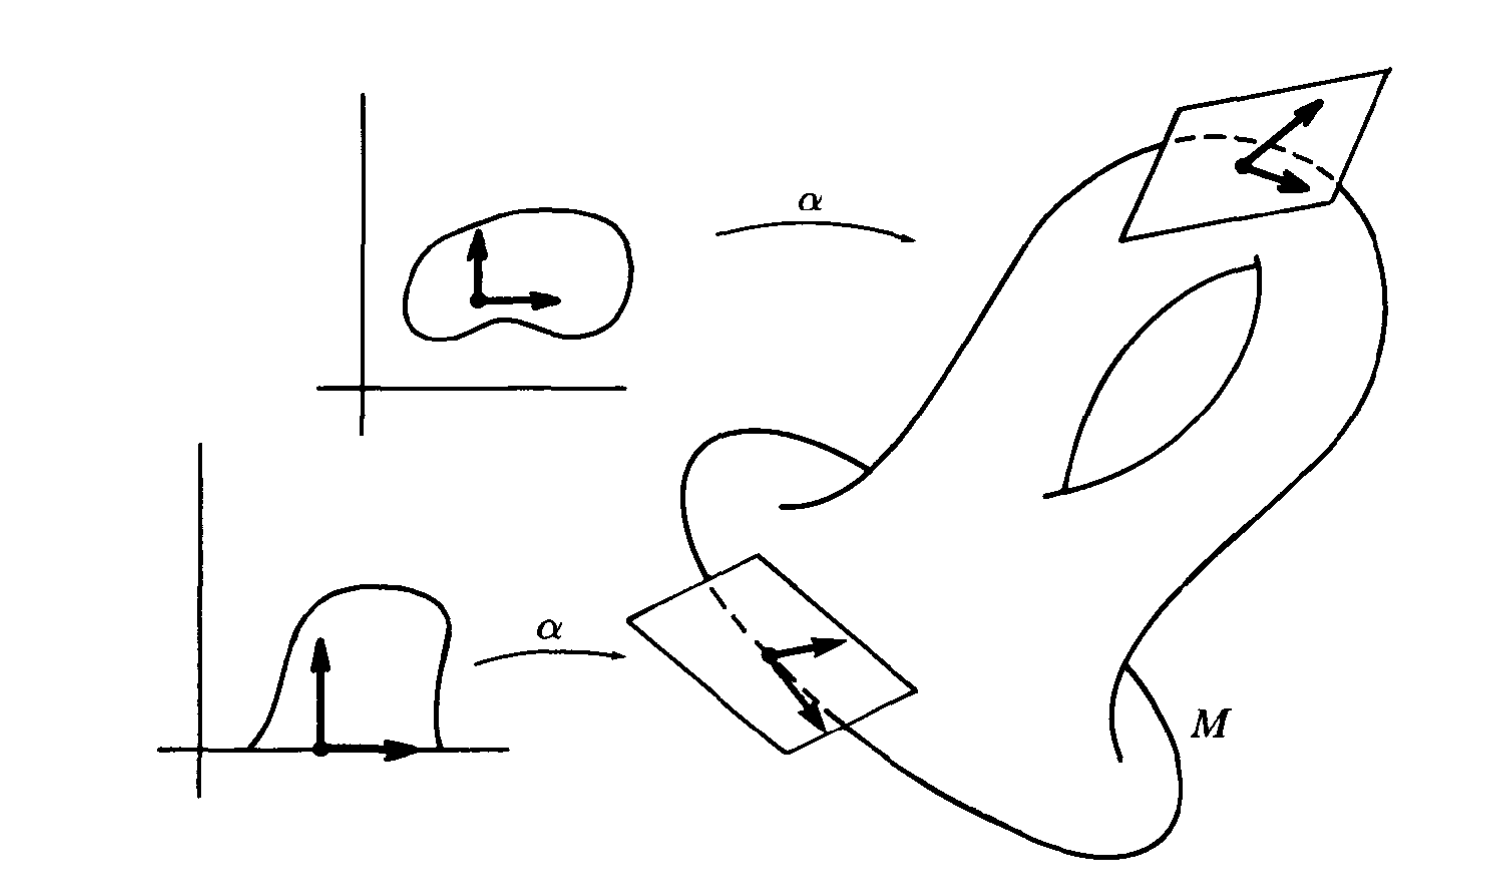
\includegraphics[scale=0.45]{images/Screenshot 2023-03-09 at 23.13.04.png}
    \end{figure}
    \item In order to make $\mathcal{T}_p(M)$ well-defined, we need to show that $\mathcal{T}_p(M)$ is independent of the coordinate patches. Consider we have two coordinate patches that overlap, as stated in theorem\ref{transition function thm}. Let $$\alpha_0:W_1\longrightarrow W$$
    $$\alpha_1:W_1\longrightarrow W$$ be two such coordinate pathches. As stated above, $\mathcal{T}_p(M)$ is spaneed by $\{(p;\frac{\partial \alpha_0}{\partial x_j})\}$. Given an arbitrary tangent vector $(p;v)$, it can be represented as
    \begin{equation*}
        \begin{split}
            (p;v) &= \sum_{i=1}^kc_i(p;\frac{\partial \alpha_0}{\partial x_i})\\
            &= \sum_{i=1}^kc_i(p;D_i\alpha_0(x))\\
            &= (p; \sum_{i=1}^kc_iD_i\alpha_0(x))\\
        \end{split}
    \end{equation*}
    What we want to show is $v=\sum_{i=1}^kc_iD_i\alpha_0(x)$ can be written as a linear combination of $\{D_i\alpha_1(y)\}$. By the theorem\ref{transition function thm} we have $$y=(\alpha_1^{-1}\circ\alpha_0)(x)$$
    and by the chain rule, we have 
    \begin{equation*}
        \begin{split}
            D\alpha_0(x) &= D(\alpha_1\circ (\alpha_1^{-1}\circ\alpha_0))(x)\\
            &= D\alpha_1((\alpha_1^{-1}\circ\alpha_0)(x))\cdot D(\alpha_1^{-1}\circ\alpha_0)(x)\\
            &= D\alpha_1(y)\cdot D(\alpha_1^{-1}\circ\alpha_0)(x)
        \end{split}
    \end{equation*}
    We know that $D(\alpha_1^{-1}\circ\alpha_0)(x)$ is a k by k invertible matrix, let us denote it by $M$ with entries $m_{i,j}$. Also denote $D\alpha_1(y)$ by $A$ with entries $a_{i,j}$. 
    Consider the i-th column of $D\alpha_0(x)$ which is $D_i\alpha_0(x)$.
    \begin{equation*}
        \begin{split}
            D_i\alpha_0(x) &= \begin{split}
                &(a_{1,1}m_{1,i} + a_{1,2}m_{2,i}+ \cdots + a_{1,k}m_{k,i})e_1\\
                &+(a_{2,1}m_{1,i} + a_{2,2}m_{2,i}+ \cdots + a_{2,k}m_{k,i})e_2\\
                &\cdots \\
                &+(a_{n,1}m_{1,i} + a_{n,2}m_{2,i}+ \cdots + a_{n,k}m_{k,i})e_n\\
            \end{split}\\
            &= m_{1,i}D_1\alpha_1(y)+ m_{2,i}D_2\alpha_1(y)+\cdots + m_{k,i}D_k\alpha_1(y)\\
            &= \sum_{j=1}^km_{j,i}D_j\alpha_1(y)
        \end{split}
    \end{equation*}
    Therefore, we have 
    \begin{equation*}
        \begin{split}
            v &= \sum_{i=1}^kc_iD_i\alpha_0(x)\\
            &= \sum_{i=1}^kc_i\sum_{j=1}^km_{j,i}D_j\alpha_1(y)\\
            &= \sum_{i=1}^k\sum_{j=1}^kc_im_{j,i}D_j\alpha_1(y)\\
            &= \sum_{j=1}^k\sum_{i=1}^kc_im_{j,i}D_j\alpha_1(y)\\
            &=  \sum_{j=1}^k(\sum_{i=1}^kc_im_{j,i})D_j\alpha_1(y)\\
            &= \sum_{j=1}^kc_j'D_j\alpha_1(y)
        \end{split}
    \end{equation*}
\end{itemize}

\begin{definition}
    The \underline{tangent bundle of $M$} is defined as $$\mathcal{T}(M)=\bigcup_{p\in M}\mathcal{T}_p(M)$$
    We should notice that this is a disjoint union.
\end{definition}
\noindent\textbf{Example}:
\begin{itemize}
    \item Consider the manifold $S^1$ in $\R^2$. For each point, we have a tangent space that is isomorphic to the tangent line at that point. So we should have infinitely many lines. 
    We should notice that $\mathcal{T}_p(S^1)=\{p\}\times \R\cong L$ where $L\subset\R^2$ is the line tangent to the point $p$. The following graph gives an example of part of the tangent bundle of $S^2$. Say $$\mathcal{T}_{p_1}(S^1),\cdots,\mathcal{T}_{p_n}(S^1)$$
    \begin{figure}[H]
        \centering
        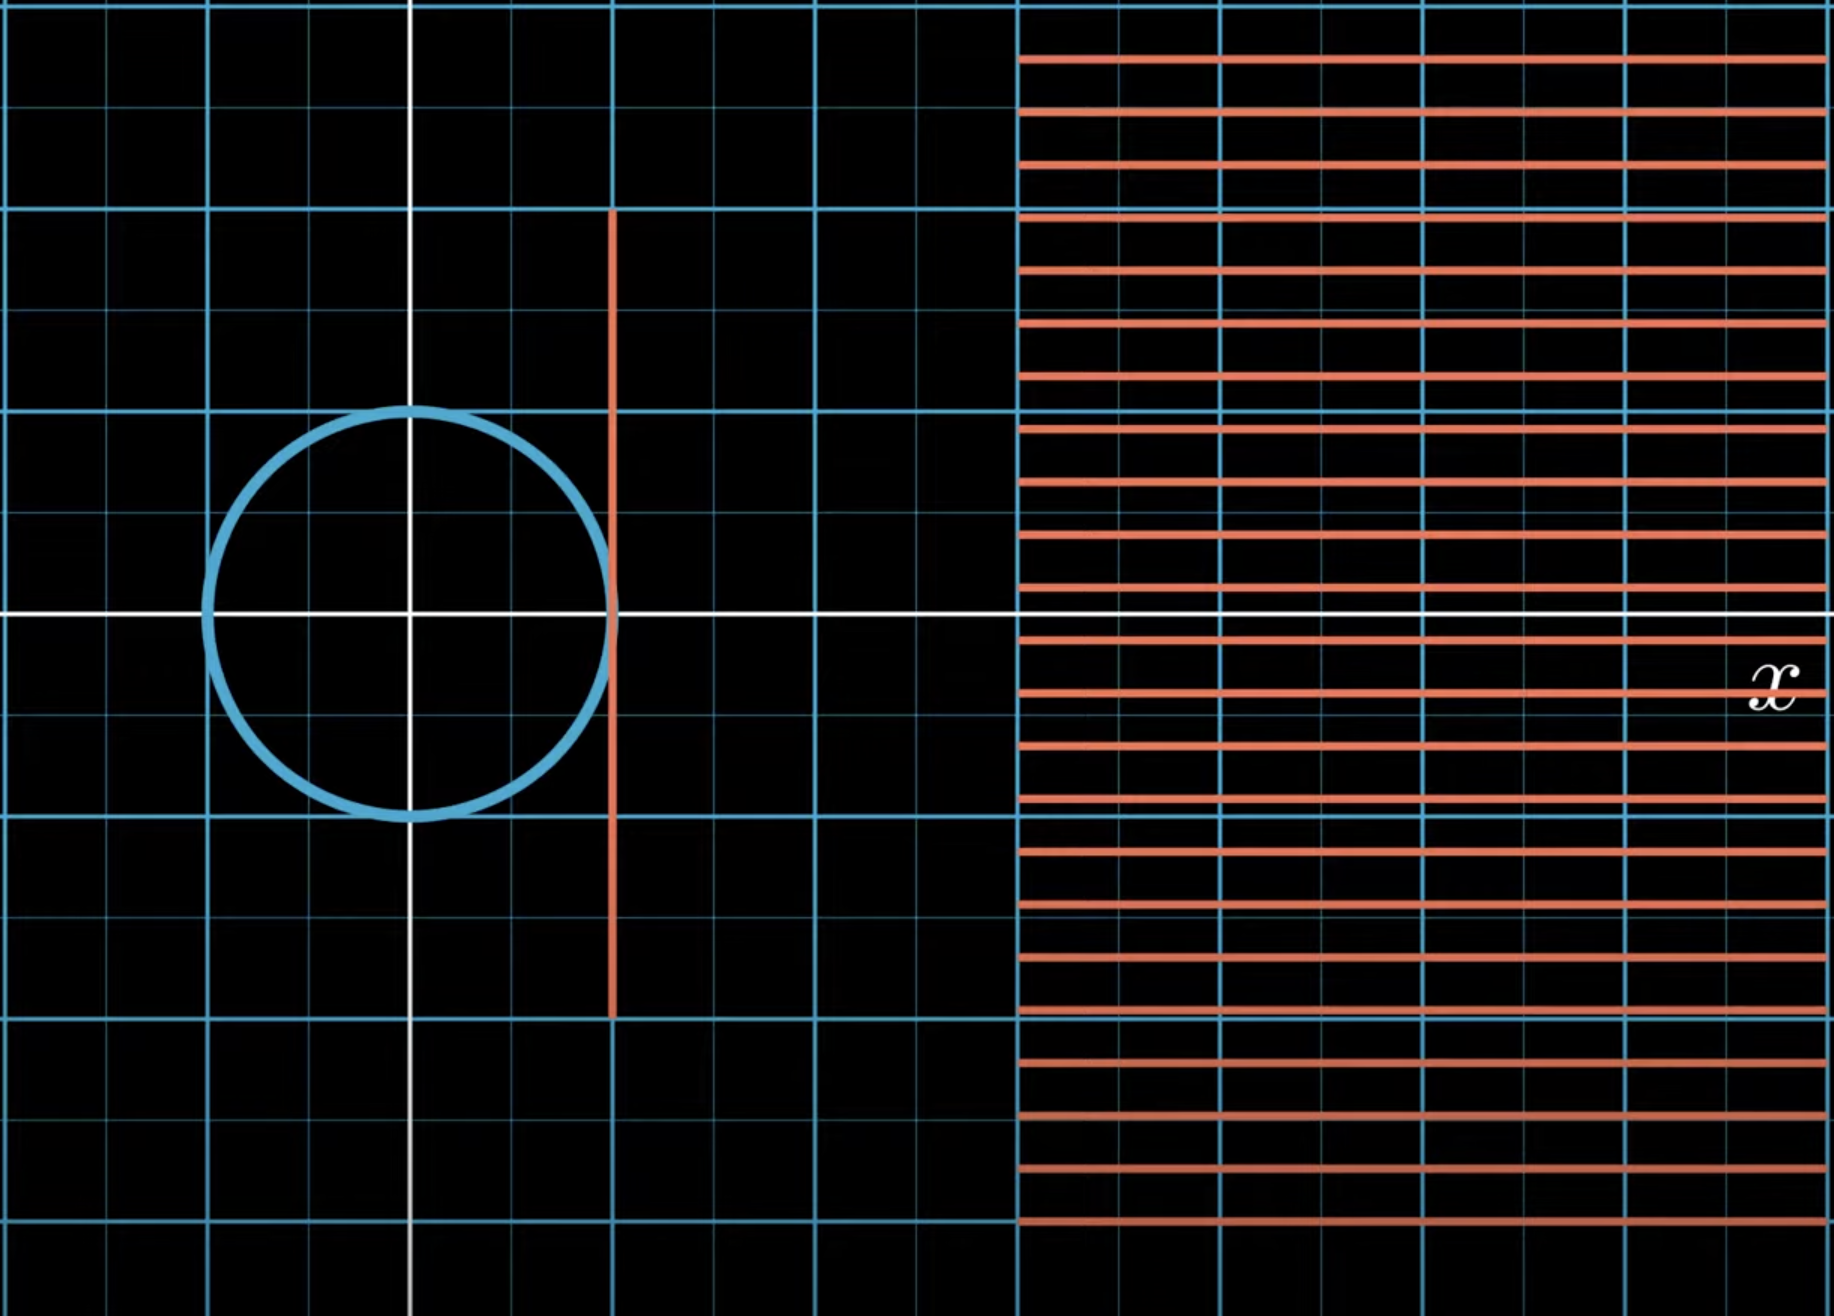
\includegraphics[scale=0.3]{images/Screenshot 2023-03-10 at 01.40.36}
    \end{figure}
    We should be aware of that each line has infinite length. We always keep in mind that $\mathcal{T}_p(S^1)$ does not live in $\R^2$ so is $\mathcal{T}(S^1)$. But we can embed each $\mathcal{T}_p(S^1)$ in $\R^2$, consider the following graph.
    \begin{figure}[H]
        \centering
        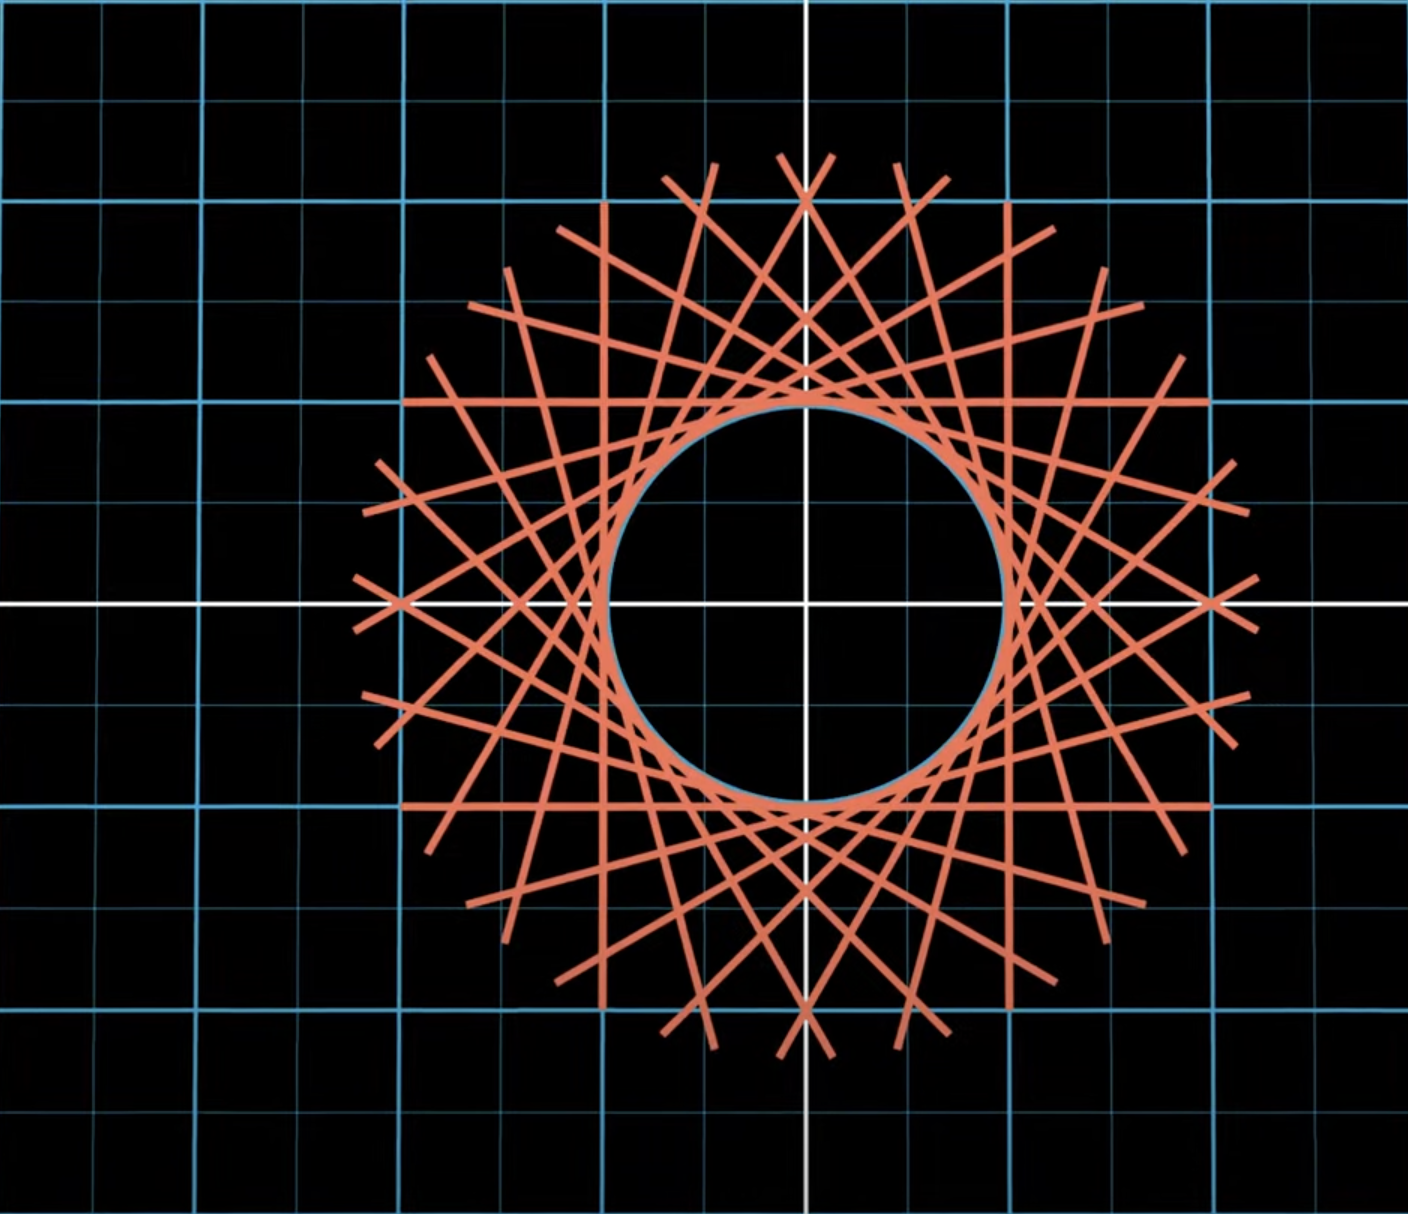
\includegraphics[scale=0.3]{images/Screenshot 2023-03-09 at 23.37.10.png}
    \end{figure}
    Someone might ask why we define the tangent space of $S^1$ at $p$ to be $\{p\}\times \R$ instead of the real tangent line $L\subset\R^2$. This is because the manifold can itself be a topological space instead of be a subspace of $\R^n$. So for a abstract manifold $S^1$, we will not have such $L\subset\R^2$. But for any $p\in S^1$, we can use the coordinate patch $\alpha$ to get the tangent space $\mathcal{T}_p(S^1)=\{p\}\times \R$.
    \item Now consider $S^2\subset \R^3$. Similarly consider a part of $\mathcal{T}(S^2)$, say $$\mathcal{T}_{p_1}(S^2),\cdots,\mathcal{T}_{p_n}(S^2)$$
    As shown in the following graph.
    \begin{figure}[H]
        \centering
        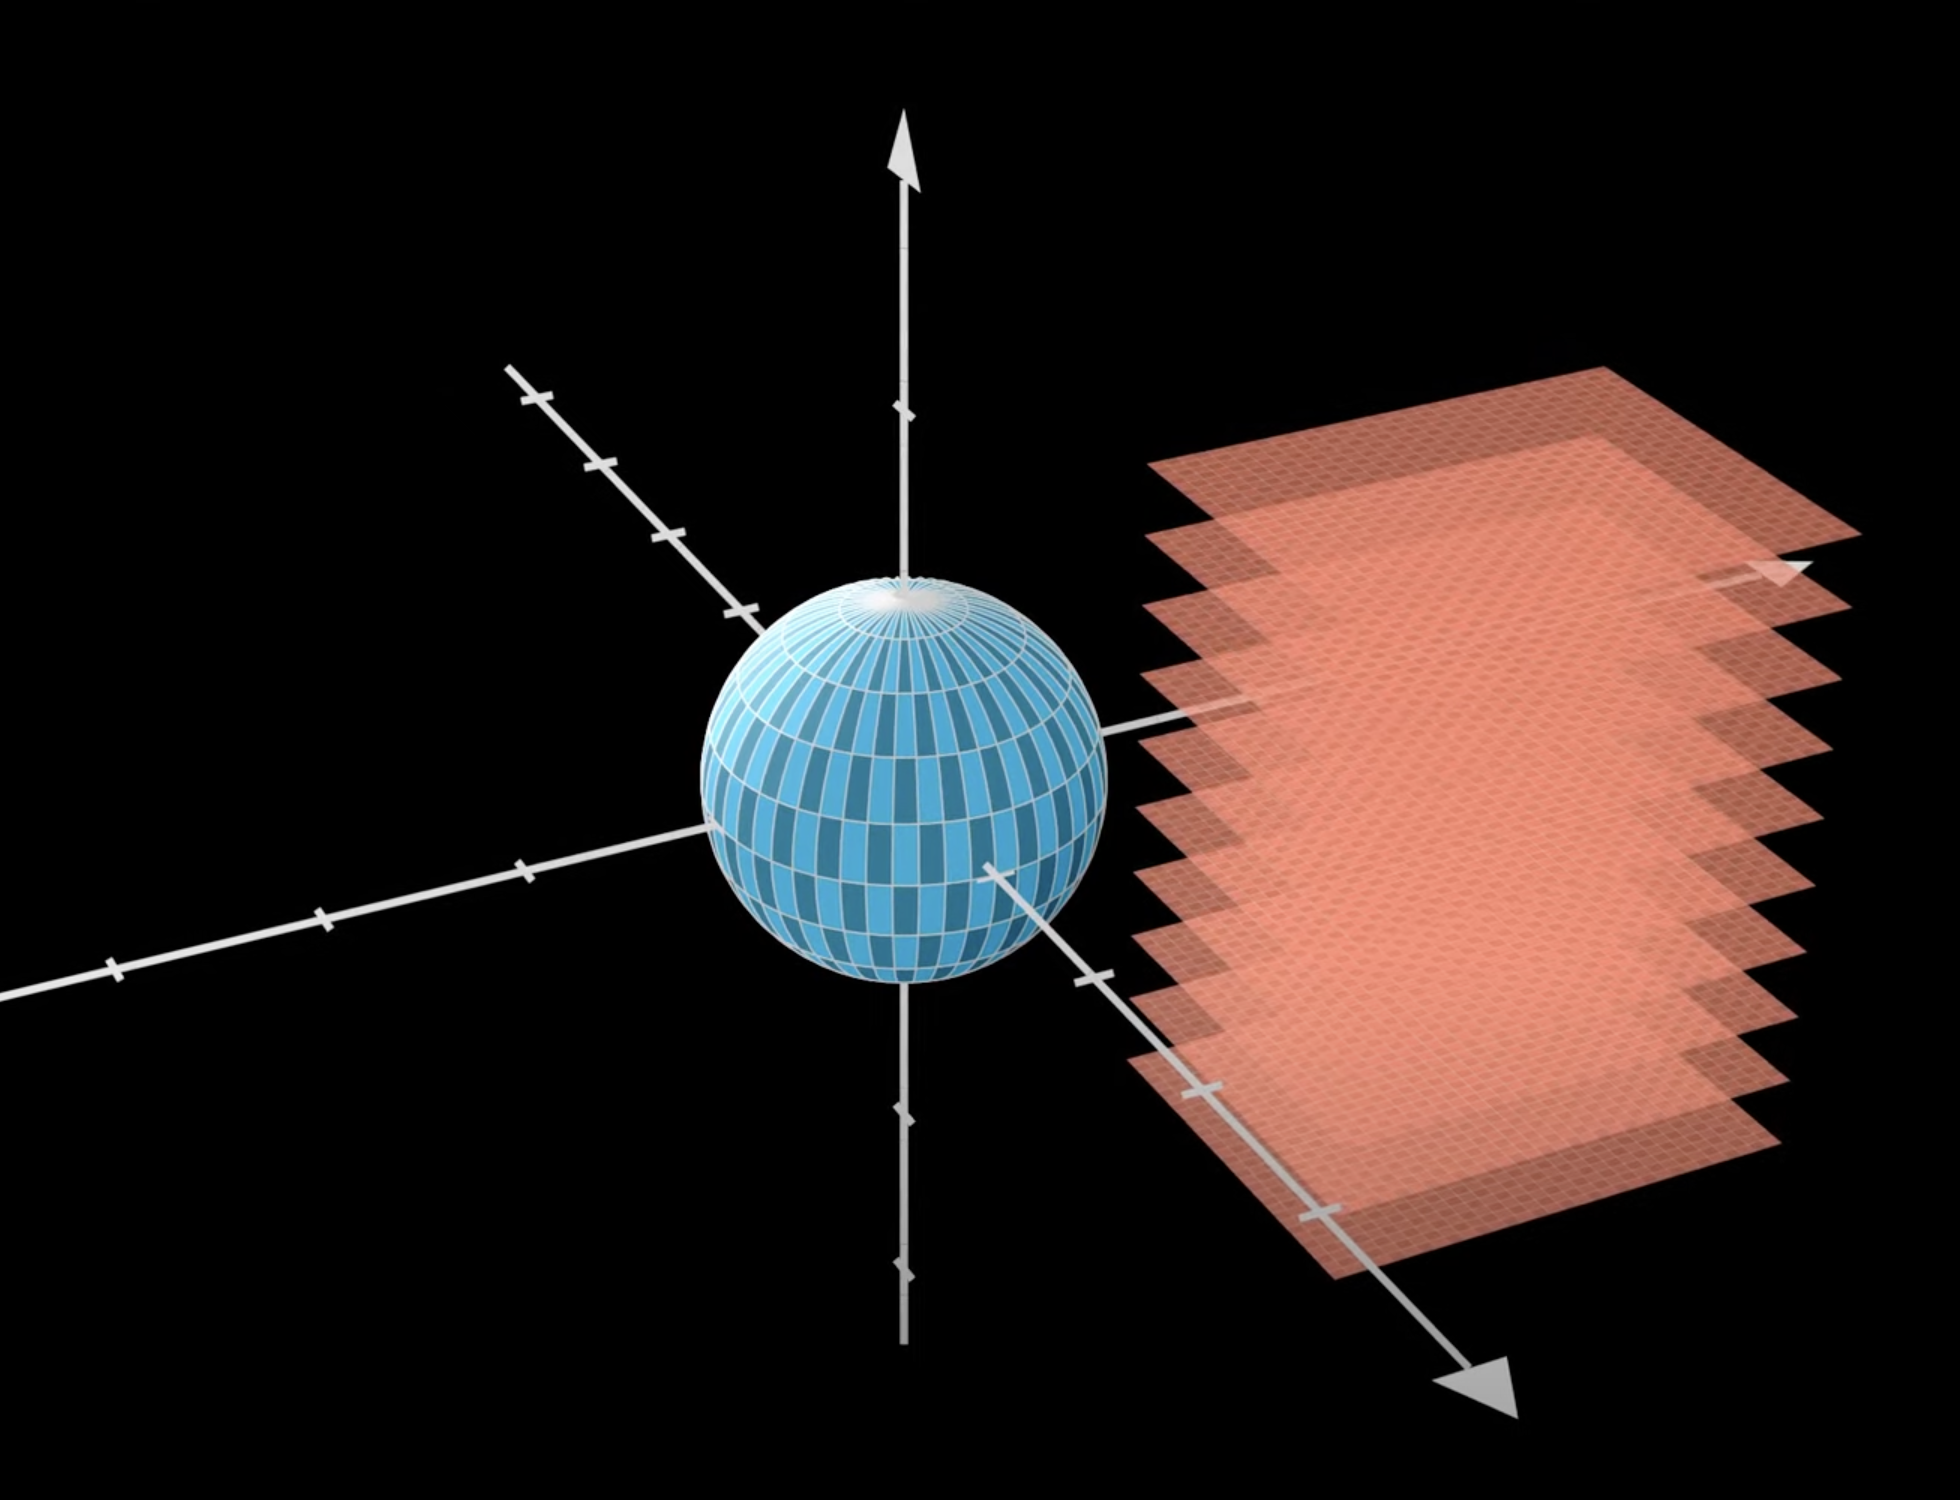
\includegraphics[scale=0.3]{images/Screenshot 2023-03-10 at 01.39.55.png}
    \end{figure}
    Each plane is infinite and is isomorphic to $\R^2$. We can embed them in to $\R^2$.
    \begin{figure}[H]
        \centering
        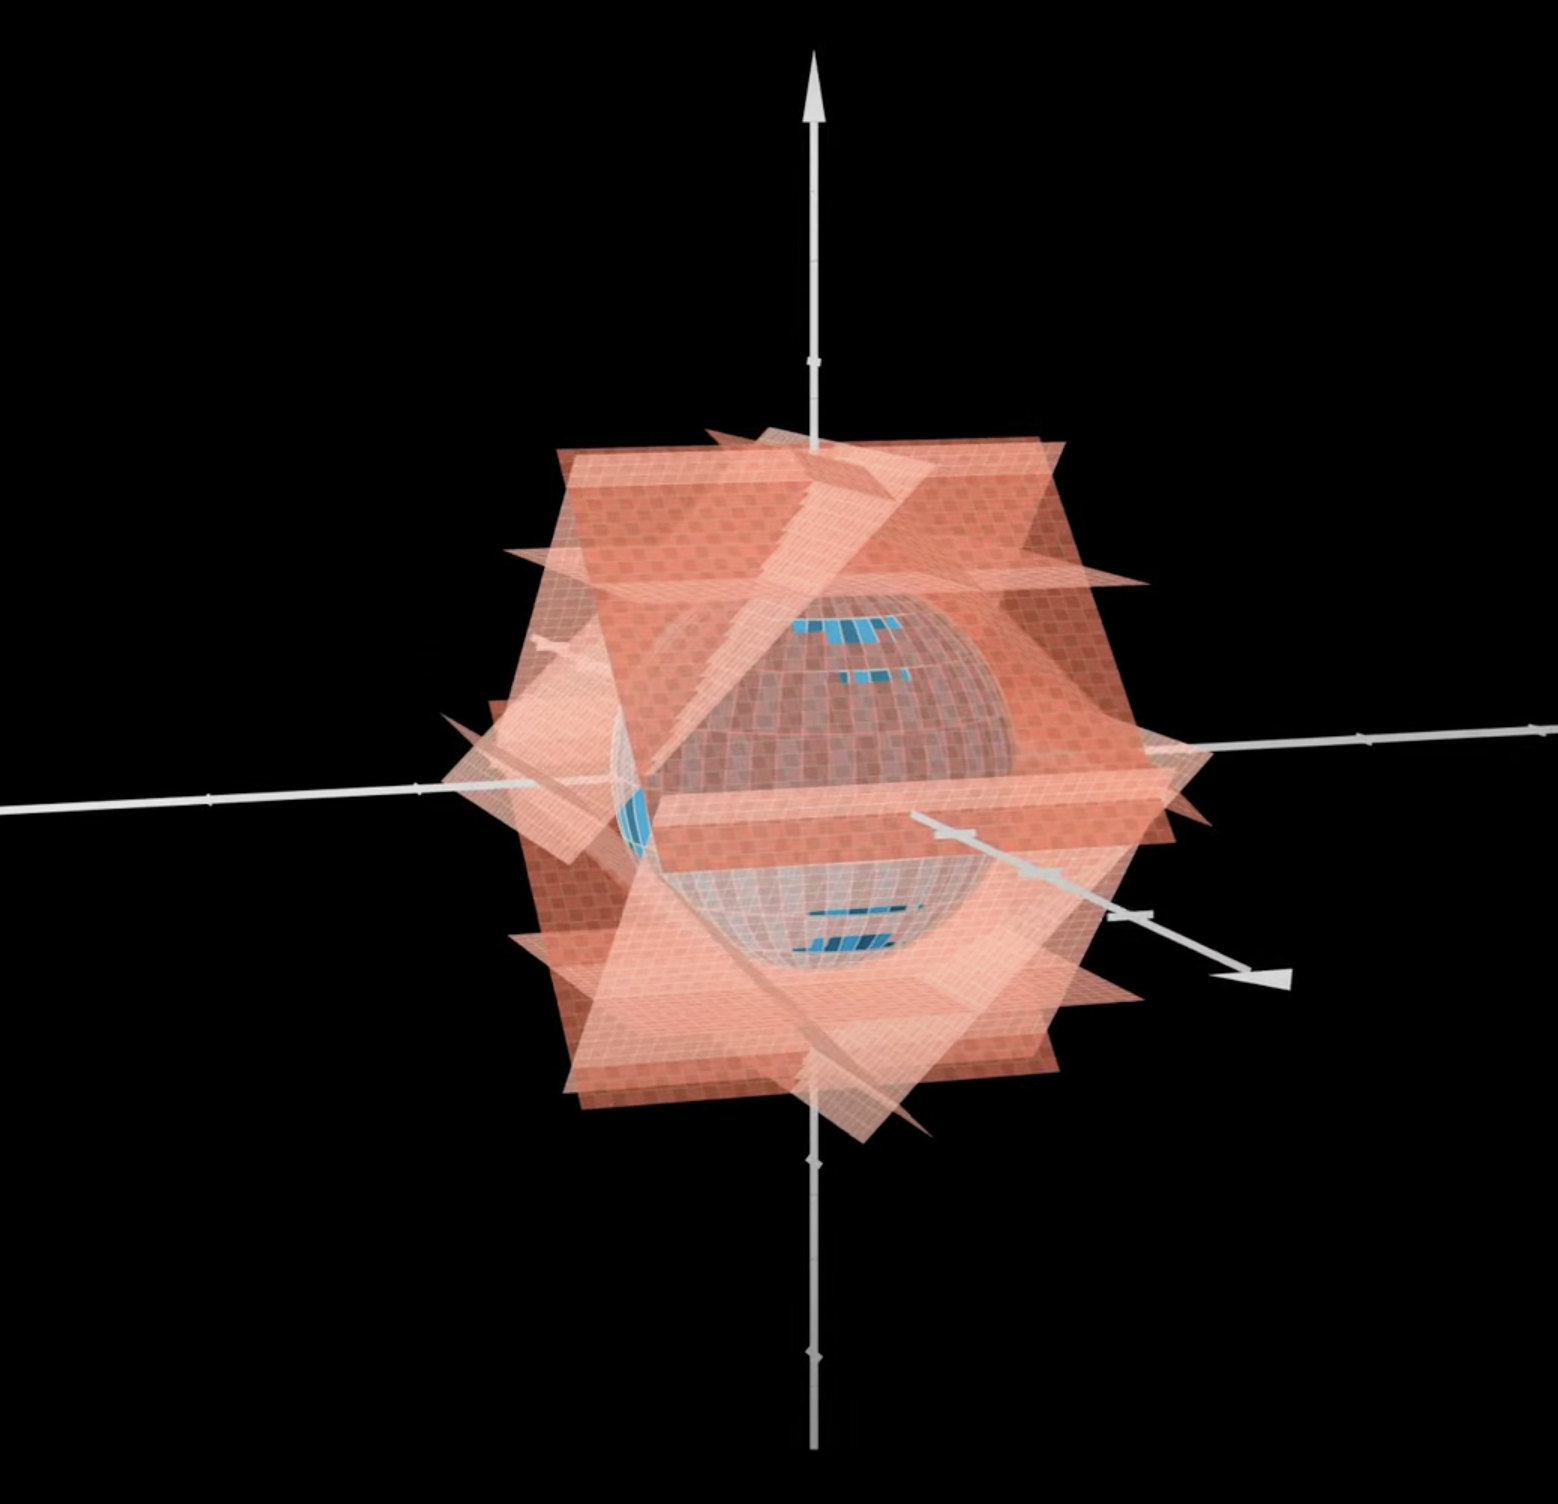
\includegraphics[scale=0.3]{images/Screenshot 2023-03-09 at 23.36.23.png}
    \end{figure}
\end{itemize}



\begin{definition}
    A \underline{tangent vector field to $M$} is a continuous function 
    $$F:M\longrightarrow \mathcal{T}(M)$$
    such that $$\forall p\in M. F(p)\in \mathcal{T}_p(M)$$
\end{definition}
\noindent\textbf{Remark}:
\begin{itemize}
    \item A vector field is intuitively just a choice of tangent vector from the tangent space at each point. In a word, we assign a direction to each point of the manifold.
\end{itemize}

\section{Differential Forms}

\begin{definition}\
    \begin{enumerate}
        \item Let $A$ be open in $\R^n$. A \underline{k-tensor field on $A$} is a function $\omega$ assigning, to each $x\in A$, a k-tensor defined on the vector space $\mathcal{T}_x(\R^n)$.
        \begin{itemize}
            \item If we fix $x\in A$, then $\omega(x)$ is a k-tensor on $\mathcal{T}_x(\R^n)$. In other words, $\omega(x)$ is a multilinear function 
            $$\omega(x):\mathcal{T}_x(\R^n)\times \cdots \times \mathcal{T}_x(\R^n)\longrightarrow \R$$
            We can write $$\omega(x)((x;v_1),\cdots,(x;v_k))$$
            \item If we consider $x$ as a variable, then
            we can also write $$\omega(x,(x;v_1),\cdots,(x;v_k))$$
        \end{itemize}
        If $\omega$ is of class $C^r$, we say $\omega$ is a \underline{tensor field of class $C^r$}.
        \item We call a k-tensor field in $A$, say $\omega$, a \underline{differential form of order k on $A$} or simply \underline{k-form on $A$} if for any $x\in A$, $\omega(x)$ is alternating. $$\omega(x)\in \mathcal{A}^k(\mathcal{T}_x(\R^n))$$
    \end{enumerate}
\end{definition}

\begin{definition}\
    \begin{enumerate}
        \item Let $M$ be a m-manifold in $\R^n$. A \underline{k-tensor field on $M$} is a function $\omega$ assigning, to each $x\in M$, a k-tensor defined on the vector space $\mathcal{T}_x(M)$.
        \begin{itemize}
            \item If we fix $x\in M$, then $\omega(x)$ is a k-tensor on $\mathcal{T}_x(M)$. In other words, $\omega(x)$ is a multilinear function 
            $$\omega(x):\mathcal{T}_x(M)\times \cdots \times \mathcal{T}_x(M)\longrightarrow \R$$
            We can write $$\omega(x)((x;v_1),\cdots,(x;v_k))$$
            \item If we consider $x$ as a variable, then 
            we can also write $$\omega(x,(x;v_1),\cdots,(x;v_k))$$
        \end{itemize}
        If $\omega$ is of class $C^r$, we say $\omega$ is a \underline{tensor field of class $C^r$}.
        \item We call a k-tensor field on $M$, say $\omega$, a \underline{differential form of order k on $M$} or simply \underline{k-form on $M$} if for any $x\in M$, $\omega(x)$ is alternating. $$\omega(x)\in \mathcal{A}^k(\mathcal{T}_x(M))$$
    \end{enumerate}
\end{definition}

\begin{theorem*}
    If $\omega$ is a tensor field defined on an open set $A$ of $\R^n$ containing the manifold $M$, then $\omega$ of course restricts to a tensor field defined on $M$. Conversly, any tensor field on $M$ can be extended to a tensor field defined on an open set of $\R^n$ containing $M$.
\end{theorem*}
\noindent\textbf{Remark}:
\begin{itemize}
    \item The converse part is not easy. For simplicity, we restrict ourselves in the textbook to tensor field that are defined on open sets of $\R^n$.
\end{itemize}

\begin{definition}
    Let $\{e_1,\cdots,e_n\}$ be the usual basis for the space $\R^n$. We define the \underline{usual basis for $\mathcal{T}_x(\R^n)$} to be the list $$\{(x;e_1),\cdots,(x;e_n)\}$$
\end{definition}

\begin{definition}\
    \begin{enumerate}
        \item The \underline{elementary 1-forms on $\R^n$} $\{\tilde{\phi_1},\cdots,\tilde{\phi_n}\}$ are defined as
        \begin{equation*}
            \tilde{\phi_i}(x)(x;e_j)=\begin{cases}
                1 \text{ if }i=j\\
                0 \text{ if }i\neq j
            \end{cases}
        \end{equation*}
        \item The \underline{elementary k-forms on $\R^n$} $\{\tilde{\psi_I}\}$, where $I=(i_1,\cdots,i_k)$ is an ascending k-tuple, are defined as 
        \begin{equation*}
            \tilde{\psi_I}(x)= \tilde{\phi_{i_1}}(x)\wedge \cdots \wedge \tilde{\phi_{i_k}}(x)
        \end{equation*}
    \end{enumerate}
\end{definition}

\noindent\textbf{Remark}:
\begin{itemize}
    \item It is clear that $\{\tilde{\phi_1},\cdots,\tilde{\phi_n}\}$ is the basis for the vector space $\mathcal{L}^1(\mathcal{T}_x(\R^n))=\mathcal{T}^*_x(\R^n)=\mathcal{A}^1(\mathcal{T}_x(\R^n))$. 
    And $\{\tilde{\psi_I}\}$ are the basis for $\mathcal{A}^k(\mathcal{T}_x(\R^n))$.
    \item Similar to $\{\psi_I\}$ can be expressed using determinants. We have 
    $$\tilde{\psi_I}(x)((x;v_1),\cdots,(x;v_k))=\det(X_I)$$
    where the matrix $X=\begin{bmatrix}
        v_1 & \cdots & v_k
    \end{bmatrix}$ and $X_I$ means the submatrix of $X$ with row $i_1,\cdots,i_k$.
\end{itemize}

\begin{theorem}
    Let $\omega$ be a k-form on an open set $A\subset \R^n$. $\omega(x)$ can be written uniquely as the form
    $$\omega(x)=\sum_Ib_I(x)\cdot \tilde{\psi_I}(x)$$
    where $b_I(x)$ is a scalar function called the \underline{components} of $\omega$ relative to the standard elementary k-forms in $\R^n$.
\end{theorem}

\begin{corollary}
    Let $\omega$ be a k-form on the open $A\subset\R^n$. Then $\omega$ is of class $C^r$ if and only if its ${n \choose k}$ components $b_I$ are of class $C^r$ on $A$.
\end{corollary}

\begin{definition}
    For $k\geq 1$, we define the space of k-forms on open $A\subset\R^n$ as $\Omega^k(A)$.
\end{definition}

\noindent\textbf{Remark}:
\begin{itemize}
    \item Now we see the space $\Omega^k(A)$ has some kind of linear structure. One might ask if it is a vector space? The answer is yes but I think it is tricky.
    It is our desire to take $\{\tilde{\psi_I}\}$ as the basis. But now the coefficients are scalar functions instead of real numbers. So $\{\tilde{\psi_I}\}$ cannot be a basis for the vector space. If we consider $\Omega^k(A)$ as a vector space over the field $\R$, then it has  uncountably infinite dimension.
    \item But what is our intuition above? Actually, $\Omega^k(A)$ is a module over the ring of smooth functions $C^{\infty}(A)$. 
    Recall that a module over a ring is a generalization of a vector space over a field. In particular, a module is an abelian group equipped with a scalar multiplication operation that satisfies certain axioms. In the case of a module over a ring, the scalars come from the ring instead of a field. We can choose $\{\tilde{\psi_I}\}$ as a basis for this module, so we have 
    $$rank(\Omega^k(A))={n \choose k}$$
    The rank of the module, which is the number of elements in a basis for the module is the notion of dimension of certain modules over commutative rings, particularly those that are finitely generated and free. 
\end{itemize}

\begin{definition}
    As we have defined the wedge product $$\wedge:\mathcal{A}^k(V)\times \mathcal{A}^m(V)\longrightarrow\mathcal{A}^{k+m}(V)$$
    We can similarly define the wedge product for $\Omega^k(A)$. The wedge product $$\wedge:\Omega^k(A)\times\Omega^m(A)\longrightarrow\Omega^{k+m}(A)$$
    is defined as $$(\omega\wedge\eta)(x)=\omega(x) \wedge \eta(x)$$
\end{definition}

\begin{lemma}
    Let $\omega$ be k-form and $\eta$ be m-form of class $C^r$, then $\omega\wedge\eta$ is a (k+m)-form of class $C^r$.
\end{lemma}

\begin{definition}
    We have defined $\Omega^k(A)$ for $k\geq1$. Now we generalize to $k=0$. We define $\Omega^0(A)$ to be the space of scalar valued functions of class $C^{\infty}$. $f\in\Omega^0(A)$ is called a \underline{differential form of order 0} or \underline{0-form}. 
    And we define $$(f\wedge g)=f(x)\cdot g(x)$$ $$(f\wedge \omega)(x)=f(x)\cdot \omega(x)$$
\end{definition}
\noindent\textbf{Remark}:
\begin{itemize}
    \item The wedge product of 0-form with k-form follows the same properties.
\end{itemize}

\section{The Differential Operator}
In this section, we will introduce an operator $$d:\Omega^k(A)\longrightarrow\Omega^{k+1}(A)$$
We first define such operator on $\Omega^0(A)$.

\begin{definition}
    Let $A$ be open in $\R^n$. Let $f:A\longrightarrow\R$ be a function of class $C^r$. We define a 1-form $df$ on $A$ by the formula $$df(x)(x;v)=Df(x)\cdot v$$
    The 1-form $df$ is called the \underline{differential of $f$}. It is of class $C^{r-1}$ as a function of $x$ and $v$.
\end{definition}

\begin{theorem}
    The operator $d$ is linear on 0-forms $\Omega^0(A)$.
\end{theorem}

\begin{lemma}
    Let $\tilde{\phi_1},\cdots,\tilde{\phi_n}$ be the elementary 1-forms on $\R^n$. Let $\pi_i:\R^n\longrightarrow\R$ be the i-th projection function, defined by the equation $$\pi_i(x_1,\cdots,x_n)=x_i$$
    Then we have $$d\pi_i=\tilde{\phi_i}$$
\end{lemma}
\noindent\textbf{Remark}:
\begin{itemize}
    \item We will use $x_i$ to denote the projection $\pi_i$, so $dx_i=\tilde{\phi_i}$.
    \item Similarly we use the notation $dx_I=\tilde{\psi_I}$ where $I$ is an increasing k-tuple. Therefore we have the expression $$dx_I=dx_{i_1}\wedge\cdots\wedge dx_{i_k}$$
    And the general k-form can be expressed uniquely as $$\omega=\sum_Ib_Idx_I$$
    \item The forms $dx_i$ and $dx_I$ are characterized by the equations 
    $$dx_i(x)(x;v)=\lambda_i \quad \text{where }v=\lambda_1a_1+\cdots+\lambda_na_n$$
    $$dx_I(x)((x;v_1),\cdots,(x;v_k))=\det(X_I) \quad \text{where } X=\begin{bmatrix}
        v_1 & \cdots & v_k
    \end{bmatrix}$$
    \item For convenience, we extend such notation to arbitrary k-tuple.
\end{itemize}

\begin{theorem}
    Let $A$ be open in $\R^n$. Let $f:A\longrightarrow\R$ be of class $C^r$. Then we have 
    $$df=(D_1f)dx_1+\cdots+(D_nf)dx_n$$
    In Leibnitz's notation, this equation takes the form 
    $$df=\frac{\partial f}{\partial x_1}dx_1+\cdots +\frac{\partial f}{\partial x_n}dx_n$$
\end{theorem}

\noindent\textbf{Remark}:
\begin{itemize}
    \item As you can see, both $df$ and $Df$ give you the same result for the directional derivative. The relationship between them is that $df$ can be thought of that $df$ provides a coordinate-free way of representing the information contained in the Jacobian matrix $Df$.
    \item Given the vector $v\in \R^n$. If we choose different coordinate system $(x_1,\cdots,x_n)$ and $(y_1,\cdots,y_n)$, then $v$ has different expression. But $df(x)(x;v)$ will always have the same result, it is coordinate-free.
\end{itemize}

\begin{definition}
    We define the \underline{differential operator} $d:\Omega^k(A)\longrightarrow\Omega^{k+1}(A)$ as follow: 
    Given a k-form $\omega$ on $A$, it can be written uniquely as $$\omega=\sum_If_Idx_I$$
    We define the (k+1)-form $d\omega$ by the equation $$d\omega=\sum_Idf_I\wedge dx_I$$
\end{definition}

\begin{theorem}{Properties of differential operator}
    For $k\geq0$, the differential operator $d:\Omega^k(A)\longrightarrow\Omega^{k+1}(A)$ as the following properties
    \begin{enumerate}
        \item The differential operator $d$ is linear on $\Omega^k(A)$.
        \item If $\omega\in \Omega^k(A)$ and $\eta\in \Omega^l(A)$, then $$d(\omega\wedge\eta)=d\omega\wedge\eta+(-1)^k\omega\wedge d\eta$$
        \item For every form $\omega$, we have $$d(d\omega)=0$$
    \end{enumerate}
\end{theorem}

\begin{definition}
    Let $A$ be open in $\R^n$.
    \begin{itemize}
        \item $f\in \Omega^0(A)$ is said to be \underline{exact} on $A$ if it is constant on $A$.
        \item $\omega\in\Omega^k(A)$ is said to be \underline{exact} on $A$ if there is a (k-1)-form $\theta$ on $A$ such that $$\omega=d\theta$$
    \end{itemize}
\end{definition}

\begin{definition}
    A k-form $\omega$ on $A$ with $k\geq0$ is said to be \underline{closed} if $d\omega=0$.
\end{definition}

\begin{theorem*}\
    \begin{itemize}
        \item If the k-form $\omega$ is exact, then it is closed.
        \item If the k-form $\omega$ is closed and $A$ is a star-convex subset in $\R^n$, then $\omega$ is exact.
    \end{itemize}
\end{theorem*}
\noindent\textbf{Remark}:
\begin{itemize}
    \item We know that the whole space $\R^n$ is star-convex in itself.
    \item If every closed k-forms on $A$ is exact on $A$, then we call $A$ is \underline{homologically trivial in dimension $k$}.
\end{itemize}
\noindent\textbf{Example}:
\begin{itemize}
    \item Let $A$ be an open set in $\R^2$ defined as $$A=\{(x,y):x\neq 0\}$$
    We defined the function $f:A\longrightarrow\R$ by $$f(x,y)=\frac{x}{|x|}$$
    $f$ is a closed 0-form on $A$ because $f$ is of class $C^{\infty}$ on $A$ and $df=0$ on $A$. But $f$ is not exact because it is not a constant.
    \item In MAT267, we say the differential equation $$P(x,y)dx+Q(x,y)dy=0$$
    is exact if there is a function $f$ such that $$P=\frac{\partial f}{\partial x}$$ $$Q=\frac{\partial f}{\partial y}$$
    In our terminology, this means that the 1-form $Pdx+Qdy$ is the differential of a 0-form $f$. And $f$ is exact because $$df=Pdx+Qdy=0$$
\end{itemize}

\section{Gradient, Divergence and Curl}

\begin{definition}
    Let $A$ be open in $\R^n$. Let $f:A\longrightarrow\R$ be a scalar field in $A$. 
    We define a corresponding (tangent) vector field in $A$, called the \underline{gradient} of $f$ by the equation 
    $$(\text{grad }f)(x)=(x;D_1f(x)e_1+\cdots+D_nf(x)e_n)$$
\end{definition}
\noindent\textbf{Remark}:
\begin{itemize}
    \item Recall we have defined the gradient for $f:\R^3\longrightarrow\R$ as 
    $$\nabla f(x)=D_1f(x)e_1+D_2f(x)e_2+D_3f(x)e_3$$
    It represents the direction of the steepest increase of $x$. We now generalize to $f:\R^n\longrightarrow\R$. 
\end{itemize}

\begin{definition}
    Given a vector field $g:A\subset \R^n\longrightarrow\R^n$, we have a corresponding (tangent) vector field $G(x)=(x;g(x))$. 
    We now define a corresponding scalar field in $A$, called the \underline{divergence} of $G$ as 
    $$(\text{div }G)(x)=D_1g_1(x)+\cdots+D_ng_n(x)$$
\end{definition}
\noindent\textbf{Remark}:
\begin{itemize}
    \item Consider air as it is heated or cooled. The velocity of the air at each point defines a vector field. While air is heated in a region, it expands in all directions, and thus the velocity field points outward from that region. The divergence of the velocity field in that region would thus have a positive value. While the air is cooled and thus contracting, the divergence of the velocity has a negative value.
    \item Now let us go back to $g:A\subset\R^3\longrightarrow\R^3$. Sometimes, for simplicity, we do not consider the tangent space. In that case $G(x)=g(x)$ and we use the notation $$\nabla \cdot G(x)=D_1G_1(x)+D_2G_2(x)+D_3G_3(x)$$
    \item Consider $V:\R^2\longrightarrow\R^2$ be the vector field in our simple setting. We can use a graph to get an intuition.
    \begin{figure}[H]
        \centering
        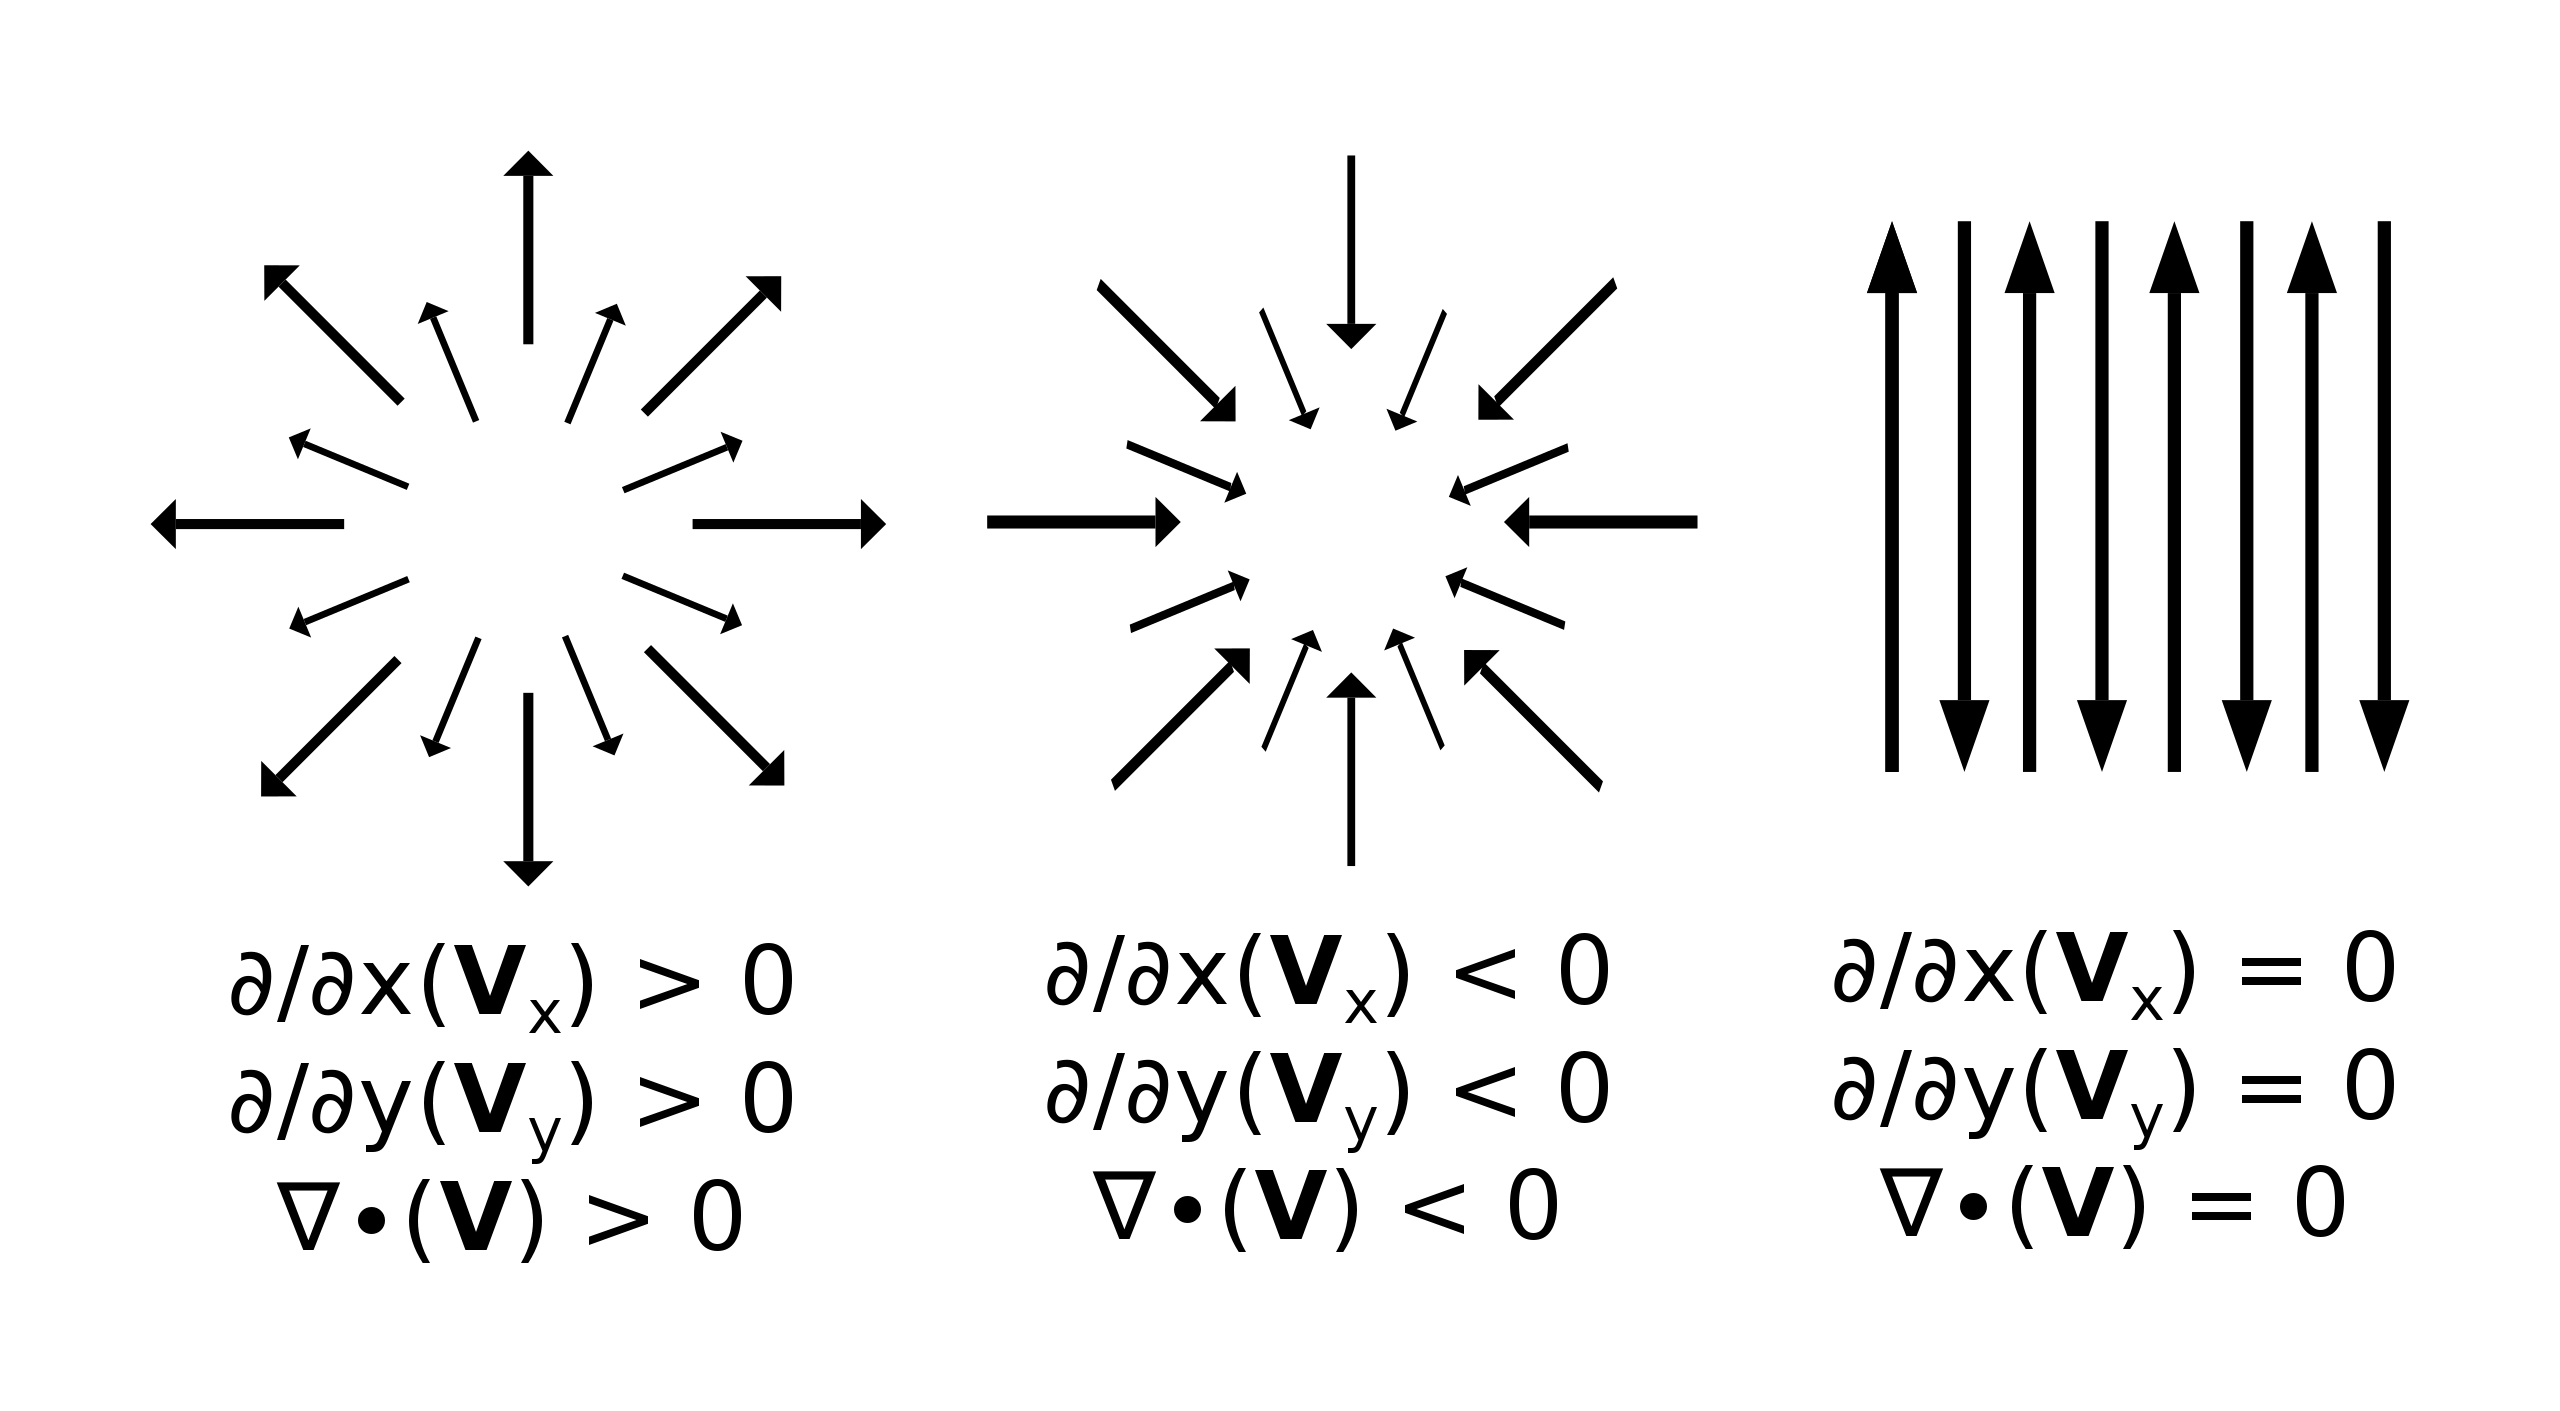
\includegraphics[scale=0.1]{images/2560px-Divergence_(captions).svg.png}
    \end{figure}
\end{itemize}

\begin{theorem}
    Let $A$ be an open set in $\R^n$. We define vector space isomorphisms
    $$\alpha_0f=f$$
    $$\alpha_1F=\sum_{i=1}^nf_idx_i$$
    $$\beta_{n-1}G=\sum_{i=1}^n(-1)^{i-1}g_idx_1\wedge\cdots \wedge\widehat{dx_i}\wedge\cdots\wedge dx_n$$
    $$\beta_nh=hdx_1\wedge\cdots\wedge dx_n$$
    And the following diagram commutes.
    \begin{figure}[H]
        \centering
        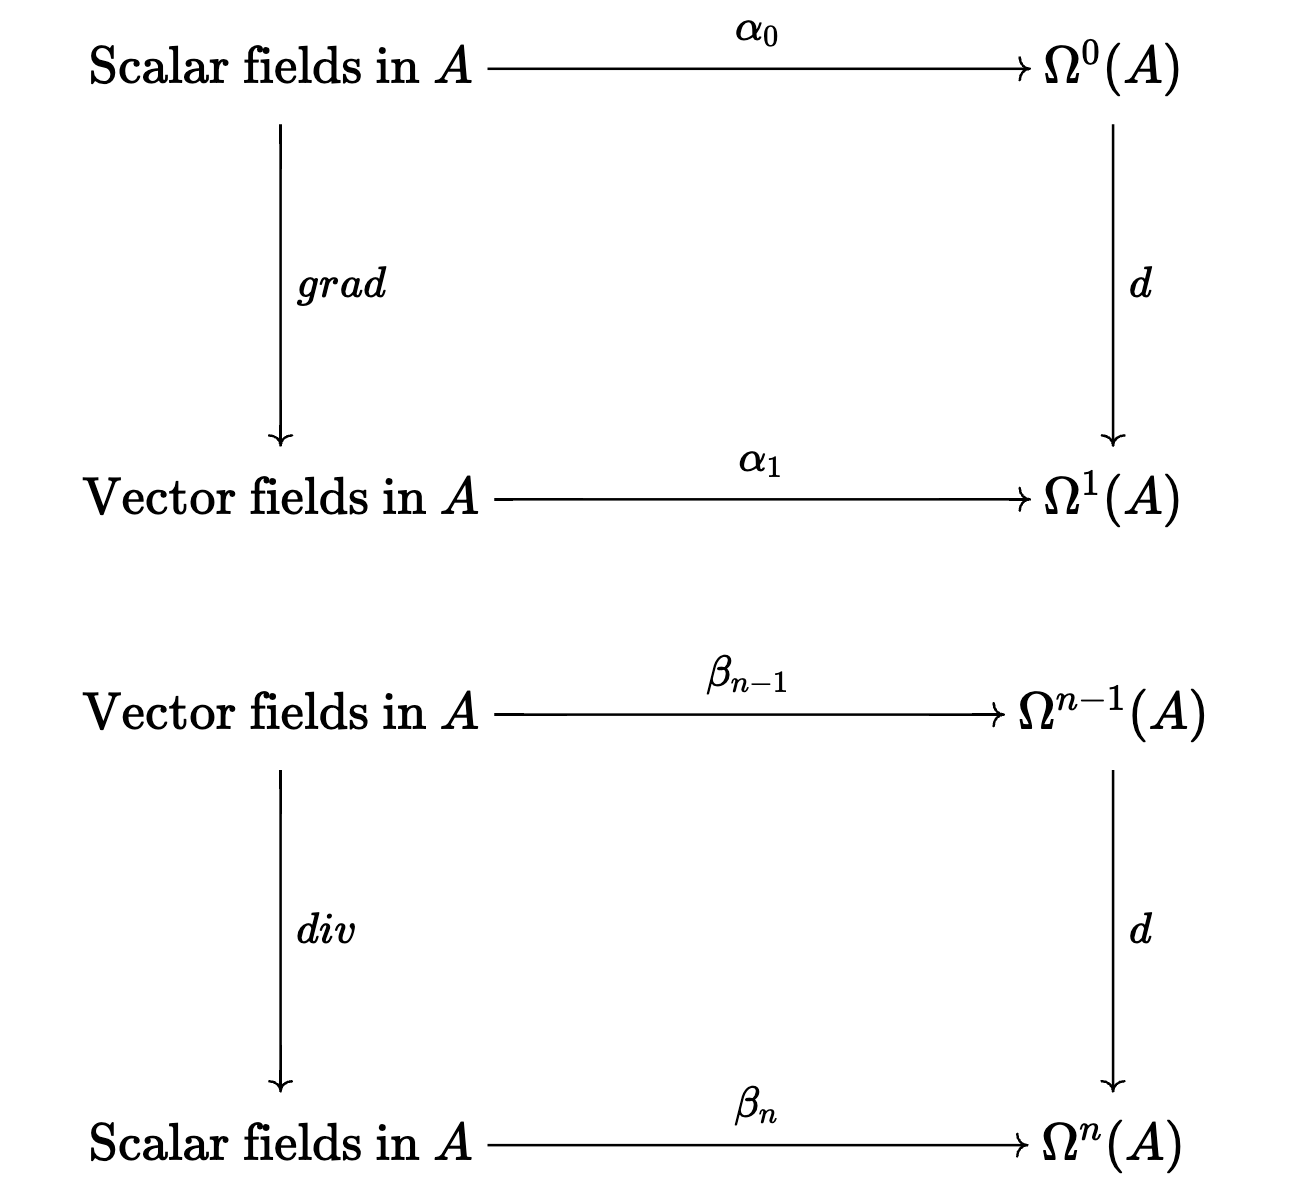
\includegraphics[scale=0.4]{images/Screenshot 2023-03-30 at 15.54.52.png}
    \end{figure}
\end{theorem}

\begin{definition}
    Given a vector field $f:A\subset\R^3\longrightarrow\R^3$, we have a corresponding (tangent) vector field $F(x)=(x;f(x))$. 
    We now define another (tangent) vector field, called the \underline{curl} of $F$ by 
    $$(\text{curl }F)(x)=(x;(D_2f_3-D_3f_2)e_1+(D_3f_1-D_1f_3)e_2+(D_1f_2-D_2f_1)e_3)$$
\end{definition}
\noindent\textbf{Remark}:
\begin{itemize}
    \item In vector calculus, the curl is a vector operator that describes the infinitesimal circulation of a vector field in three(or two)-dimensional Euclidean space. The curl at a point in the field is represented by a vector whose length and direction denote the magnitude and axis of the maximum circulation. The curl of a field is formally defined as the circulation density at each point of the field.
    \item Similarly to divergence, we sometimes consider $F(x)=f(x)$ and use the notation $$\nabla\times F(x)=(D_2F_3-D_3F_2)e_1+(D_3F_1-D_1F_3)e_2+(D_1F_2-D_2F_1)e_3$$
    \item In the simple setting, consider the vector field $F(x,y,z)=(y,-x,z)$ which means for each vector, we rotate it 90 degree clockweise.
    \begin{figure}[H]
        \centering
        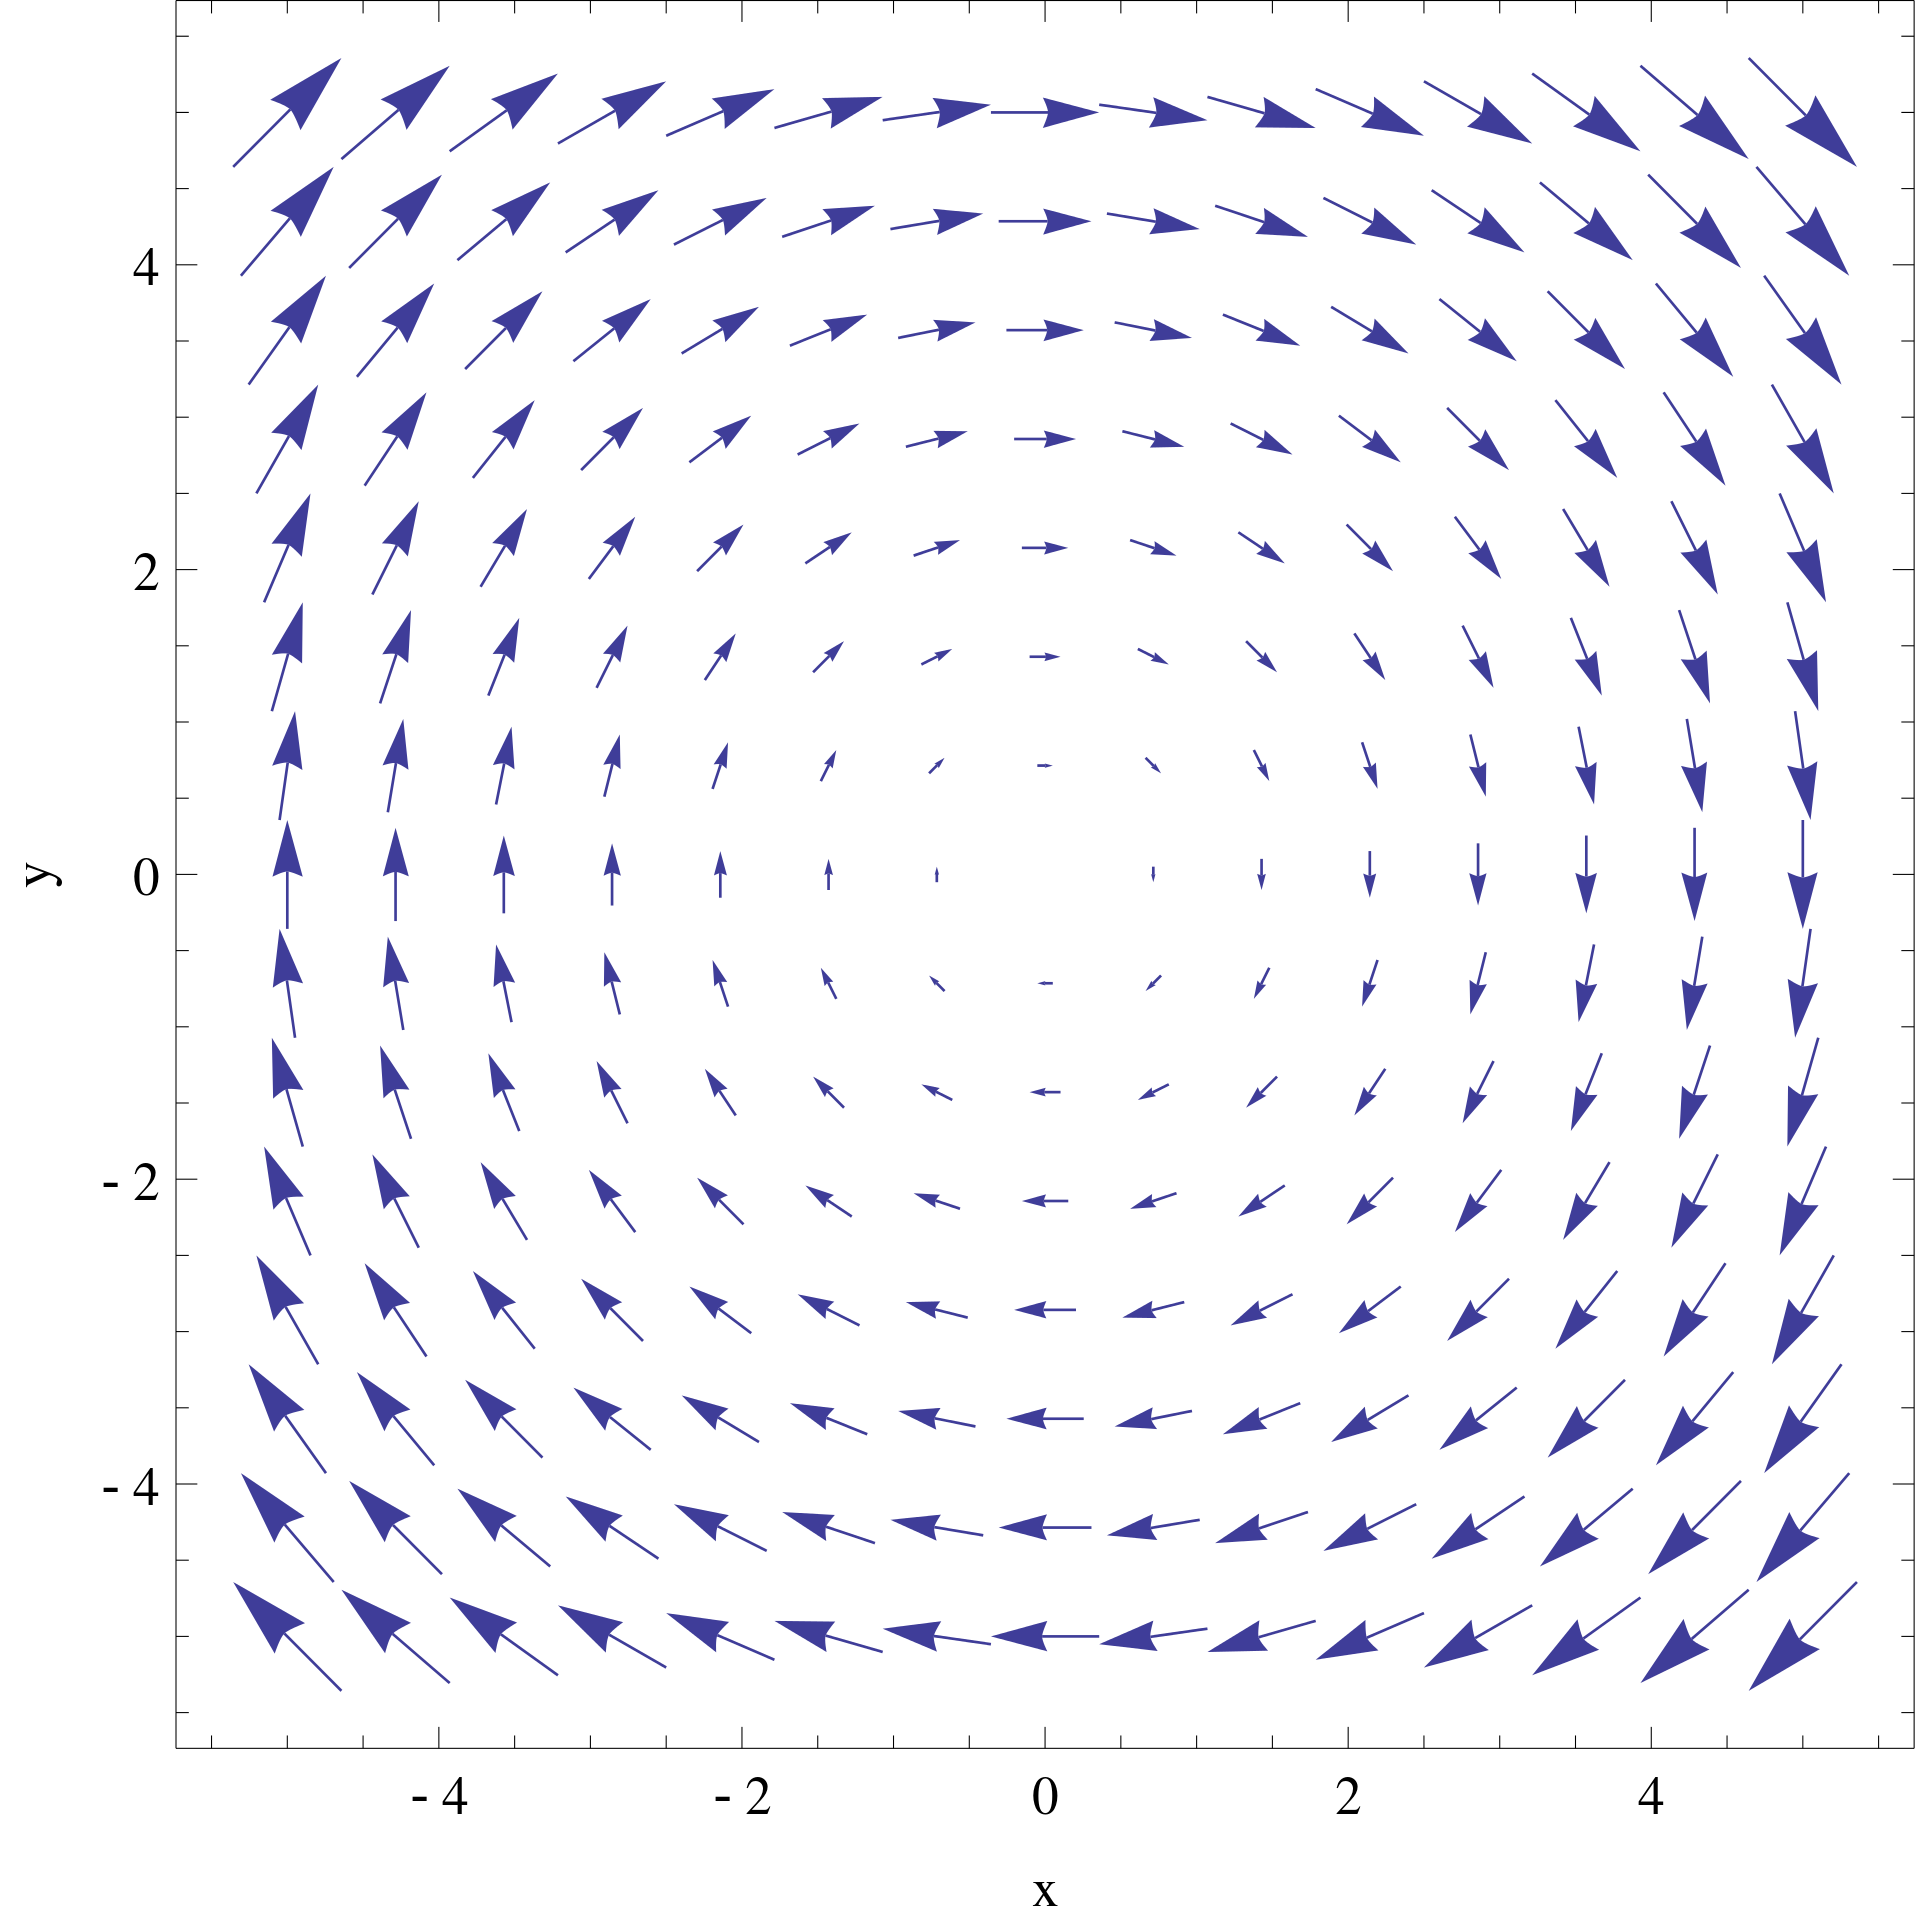
\includegraphics[scale=0.1]{images/Uniform_curl.svg.png}
        \caption{The vector field of $F(x,y,z)=(y,-x,z)$ with $z=0$}
    \end{figure}
    \begin{figure}[H]
        \centering
        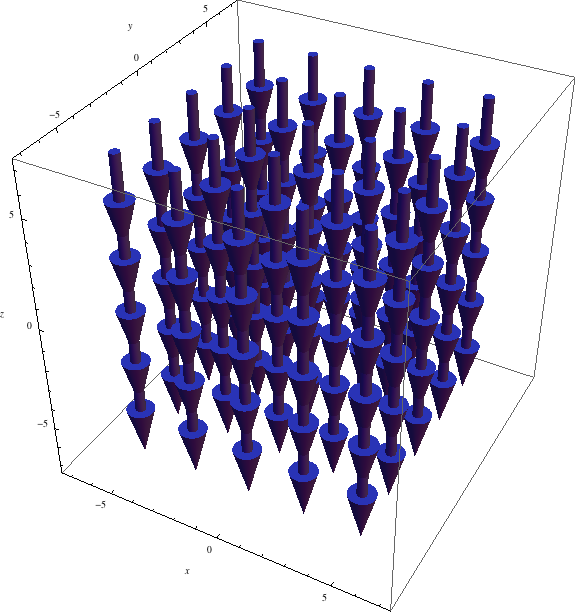
\includegraphics[scale=0.3]{images/Curl_of_uniform_curl.png}
        \caption{Image of $\nabla\times F(x,y)$}
    \end{figure}
\end{itemize}

\begin{theorem}
    Let $A$ be an open set in $\R^3$, the following diagram commutes.
    \begin{figure}[H]
        \centering
        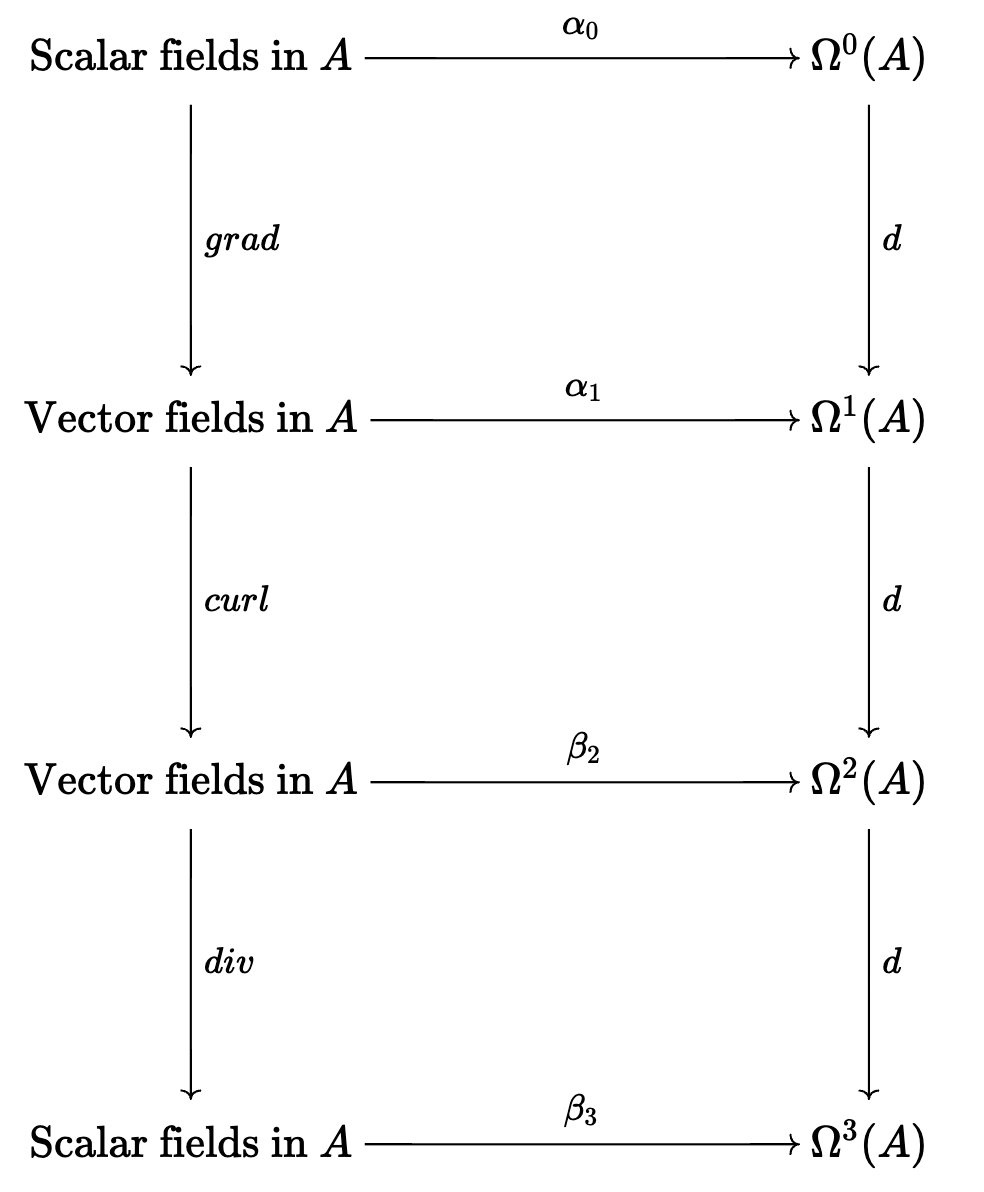
\includegraphics[scale=0.45]{images/Screenshot 2023-03-30 at 16.00.34.png}
    \end{figure}
\end{theorem}

\section{The Action of Differential Maps}

\begin{definition}
    Let $A$ be open in $\R^k$. Let $\alpha:A\longrightarrow\R^n$ be of class $C^{\infty}$. Let $B$ be an open set in $\R^n$ containing $\alpha(A)$. We now define the \underline{dual transformation of forms} $$\alpha^*:\Omega^l(B)\longrightarrow\Omega^l(A)$$
    \begin{enumerate}
        \item Given a 0-form $f:B\longrightarrow\R$ on $B$, we define a 0-form on $A$ by setting $$(\alpha^*f)(x)=f(\alpha(x))$$
        \item Given a l-form $\omega\in \Omega^l(B)$, we define an l-form on $A$ by setting
        \begin{equation*}
            \begin{split}
                (\alpha^*\omega)(x)((x;v_1),\cdots,(x;v_l)) &= \omega(\alpha(x))(\alpha_*(x;v_1),\cdots,\alpha_*(x;v_l))\\
                &= \omega(\alpha(x))((\alpha(x);D\alpha(x)v_1),\cdots,(\alpha(x);D\alpha(x)v_l))
            \end{split}
        \end{equation*}
    \end{enumerate}
\end{definition}
\noindent\textbf{Remark}:
\begin{itemize}
    \item We can use the following graph to represent $\alpha^*$.
    \begin{figure}[H]
        \centering
        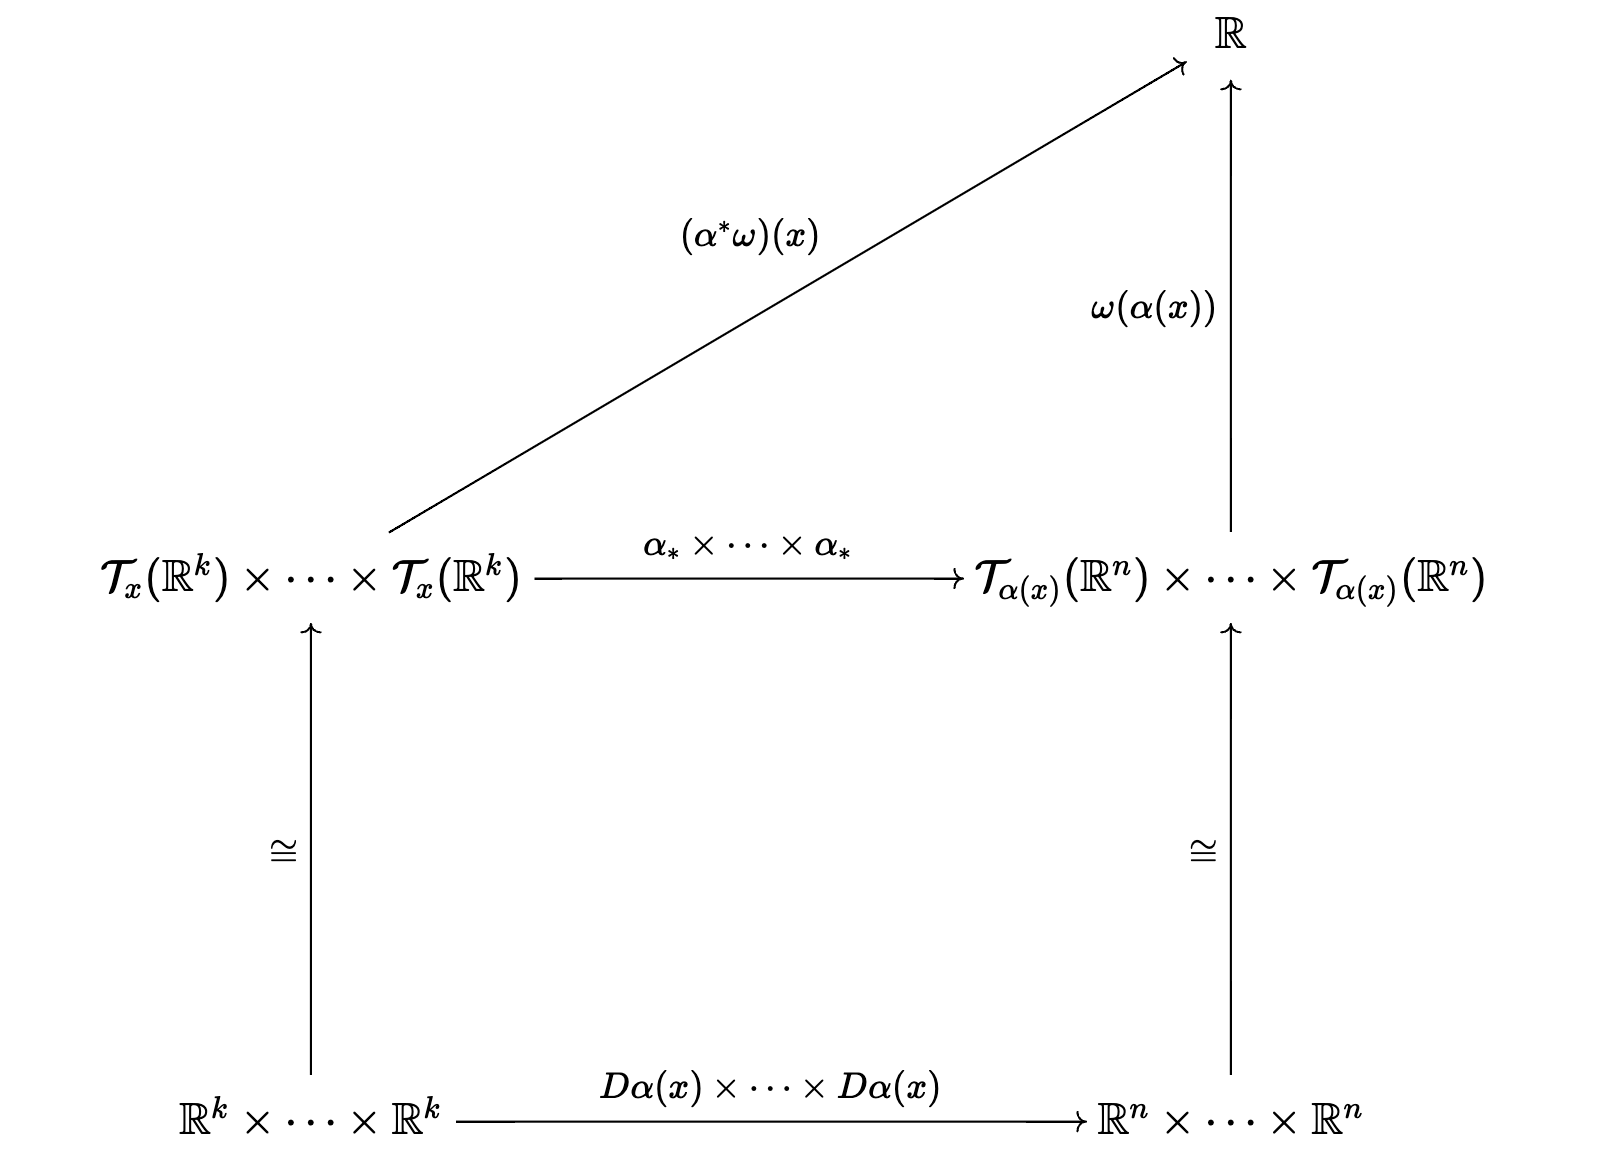
\includegraphics[scale=0.5]{images/Screenshot 2023-03-20 at 17.48.39.png}
    \end{figure}
    \item $T=\alpha_*:\mathcal{T}_x(\R^k)\longrightarrow\mathcal{T}_{\alpha(x)}(\R^n)$ is a linear transformation. Recall the dual transformation of alternating tensors. 
    $$T^*:\mathcal{A}^l(\mathcal{T}_{\alpha(x)}(\R^n))\longrightarrow\mathcal{A}^l(\mathcal{T}_x(\R^k))$$
    and it is satisfies $$T^*(\omega(\alpha(x)))=(\alpha^*\omega)(x)$$
\end{itemize}

\begin{theorem}
    Let $A$ be open in $\R^k$. Let $\alpha:A\longrightarrow\R^m$ be of class $C^{\infty}$. Let $B$ be open in $\R^m$ and containing $\alpha(A)$. 
    Let $\beta:B\longrightarrow\R^n$ be of class $C^{\infty}$. 
    Let $\omega$, $\eta$ be forms of same order defined in open $C$ in $\R^n$ containing $\beta(B)$. Let $\theta$ be another form on $C$. Then we have
    \begin{enumerate}
        \item $\beta^*(a\omega+b\eta)=a(\beta^*\omega)+b(\beta^*\eta)$
        \item $\beta^*(\omega\wedge\theta)=\beta^*\omega\wedge\beta^*\theta$
        \item $(\beta\circ\alpha)^*\omega=\alpha^*(\beta^*\omega)$
    \end{enumerate}
\end{theorem}
\noindent\textbf{Remark}:
\begin{itemize}
    \item This theorem says that the pullback operator of forms preservec the vector space structure and the wedge product.
    \item We now show it preserves the differential operator $d$.
\end{itemize}

\begin{theorem}
    Let $A$ be open in $\R^k$. Let $\alpha:A\longrightarrow\R^n$ be of class $C^{\infty}$. 
    Let $x$ denote the general point in $\R^k$ and $y$ denote the general point in $\R^n$. 
    Then $dx_i$ and $dy_i$ denote the elementary 1-forms in $\R^k$ and $\R^n$ respectively.
    \begin{enumerate}
        \item $\alpha^*(dy_i)=d\alpha_i$
        \item If $I=(i_1,\cdots,i_k)$ is an ascending k-tuple from the set $\{1,\cdots,n\}$, then $$\alpha^*(dy_I)=\det(\frac{\partial \alpha_I}{\partial x})dx_1\wedge \cdots \wedge dx_k$$
        where $$\frac{\partial \alpha_I}{\partial x}=\frac{\partial (\alpha_{i_1},\cdots,\alpha_{i_k})}{\partial (x_1\cdots,x_k)}=D\alpha(x)_I$$
    \end{enumerate}
\end{theorem}

\begin{theorem}
    Let $A$ be open in $\R^k$. Let $\alpha:A\longrightarrow\R^n$ be of class $C^{\infty}$. 
    if $\omega$ is an l-form defined in an open set of $\R^n$ containing $\alpha(A)$, then $$\alpha^*(d\omega)=d(\alpha^*\omega)$$
\end{theorem}

\begin{theorem}
    Let $A$ be open in $\R^k$. Let $\alpha:A\longrightarrow\R^n$ be of class $C^{\infty}$.
    Let $x$ denote the general point in $\R^k$ and $y$ denote the general point in $\R^n$. 
    If $I=(i_1,\cdots,i_l)$ is an ascending l-tuple from the set $\{1,\cdots,n\}$, then $$\alpha^*(dy_I)=\sum_J\det(\frac{\partial \alpha_I}{\partial x_J})dx_J$$
    Here $J=(j_1,\cdots,j_l)$ is an ascending l-tuple from the set $\{1,\cdots,k\}$, and 
    $$\frac{\partial \alpha_I}{\partial x_J}=\frac{\partial (\alpha_{i_1},\cdots,\alpha_{i_l})}{\partial (x_{j_1}\cdots,x_{j_l})}=D\alpha(x)_{I,J}$$
\end{theorem}